\documentclass[10pt]{beamer}

\linespread{1.2}
%%\usetheme{Berkeley}

\title{Electric Drive Optimization}
\author{Chong Chee Kang}
\date{\today}

\line

\begin{document}

\frame{\titlepage}

\section[Outline]{}
\frame{\tableofcontents}

\section{Introduction}

\subsection{PMBLDC}

\frame{
	\frametitle{PMBLDC}
	
	\begin{itemize}
		\item Permanent Magnet Brushless DC motor
		
		\begin{figure}
			\centering
			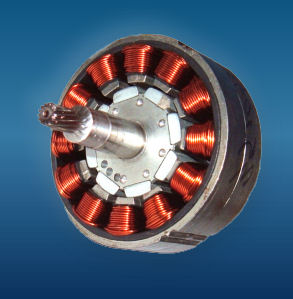
\includegraphics[width=2in]{images/bldc.jpg}
			\caption{PMBLDC motor, source: http://dev.emcelettronica.com/}
		\end{figure}
	\end{itemize}
}

\subsection{Shell Eco-Marathon}

\frame{
	\frametitle{Shell Eco-Marathon}
	
	\begin{itemize}
		\item Race for mileage, not speed
		\item Category:
		\begin{itemize}
			\item Urban Concept
			\item Protoype
		\end{itemize}
		\item plug-in electric
		\item 4 laps with 10 seconds stoppage between each lap
	\end{itemize}
}

\subsection{Problem Statement}
\frame{
	\frametitle{Problems}
	
	\begin{itemize}
		\item Types of torque produced by PMBLDC
		\begin{itemize}
			\item cogging torque
			\item reluctance torque
			\item mutual torque
		\end{itemize}
		
		\item Torque ripple
		
		\item Poor Strategy
	\end{itemize}
}
\subsection{Objectives}
\frame{
	\frametitle{Objectives}

	\begin{enumerate}
		\item To identify the output signal of the controller circuit and the hall effect sensor of the PMBLDC and develop a set of instrument for measuring the mileage of the electric vehicle.
		\item To study the track profile of Sepang North Track and create a simulation program for simulating the vehicle dynamics at the Sepang North Track.
		\item To compose a set of strategy to increase the mileage of the electric vehicle running on the Sepang North Track using the simulation program.
	\end{enumerate}
}

\section{Methodology}

\subsection{Signal Identification and Measurement System}

\frame{
	\frametitle{Signal Identification and Measurement System}
	
	\begin{figure}
		\centering
		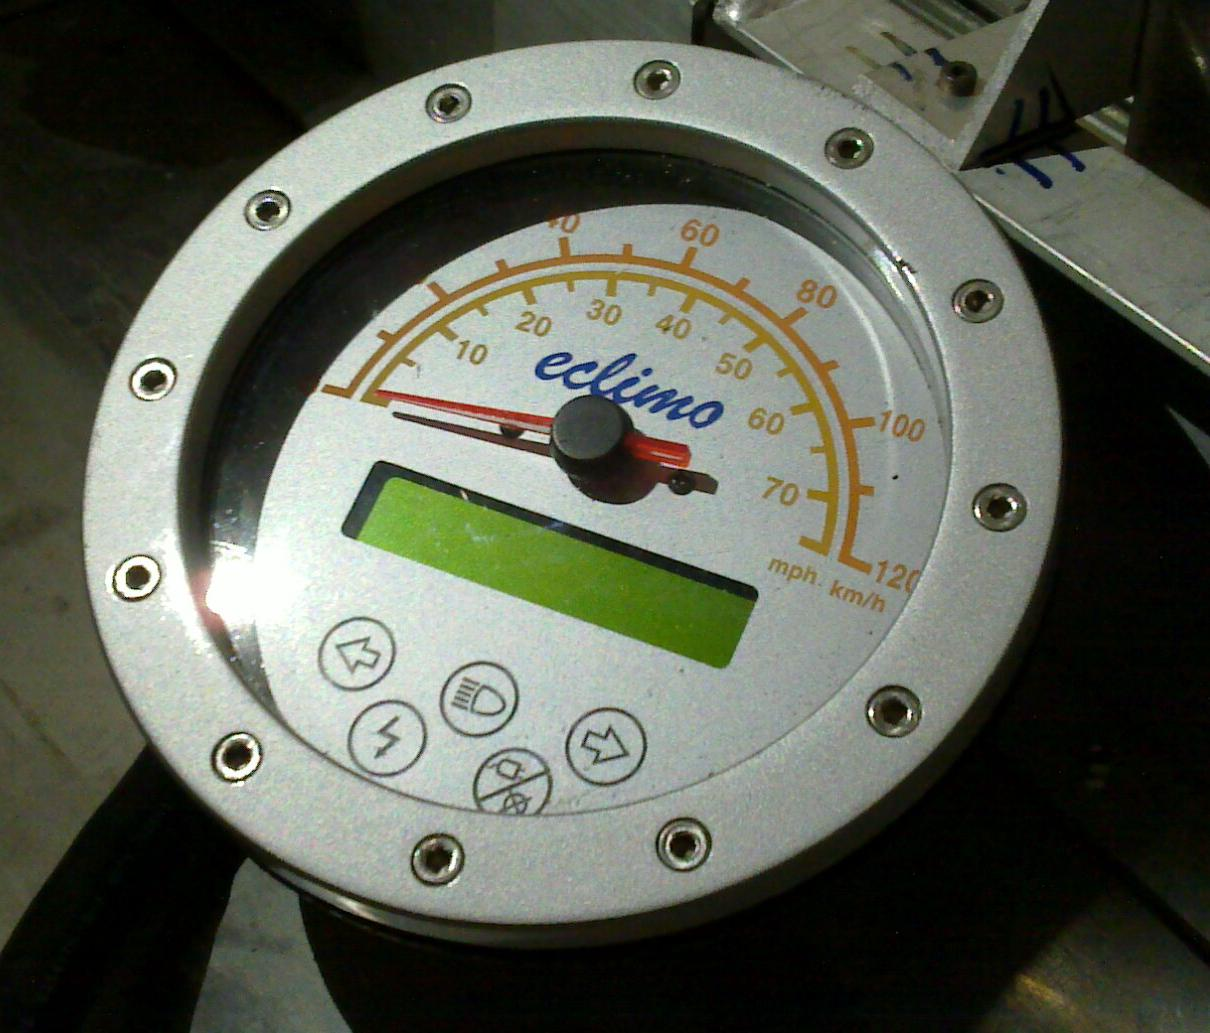
\includegraphics[width=3in]{images/speedo.jpg}
		\caption{Eclimo's speedometer}
	\end{figure}
}

\frame {
	\frametitle{Signal Identification and Measurement System}
	
	\begin{figure}
		\centering
		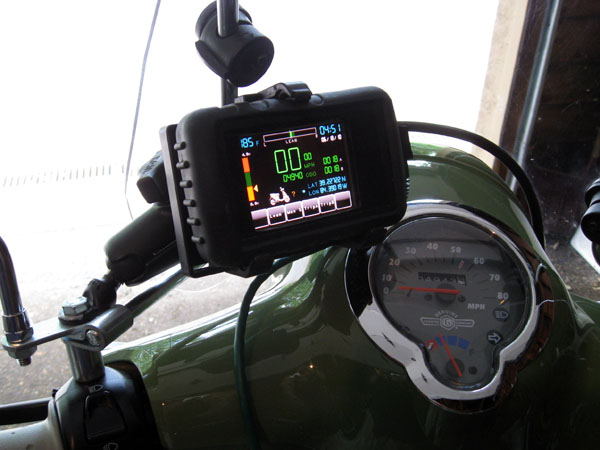
\includegraphics[width=3in]{images/scooterputer.jpg}
		\caption{Scooterputer, source: http://www.janspace.com/b2evolution/arduino.php/scooterputer}
	\end{figure}
}

\frame {
	\frametitle{Signal Identification and Measurement System}
	
	\begin{figure}
		\centering
		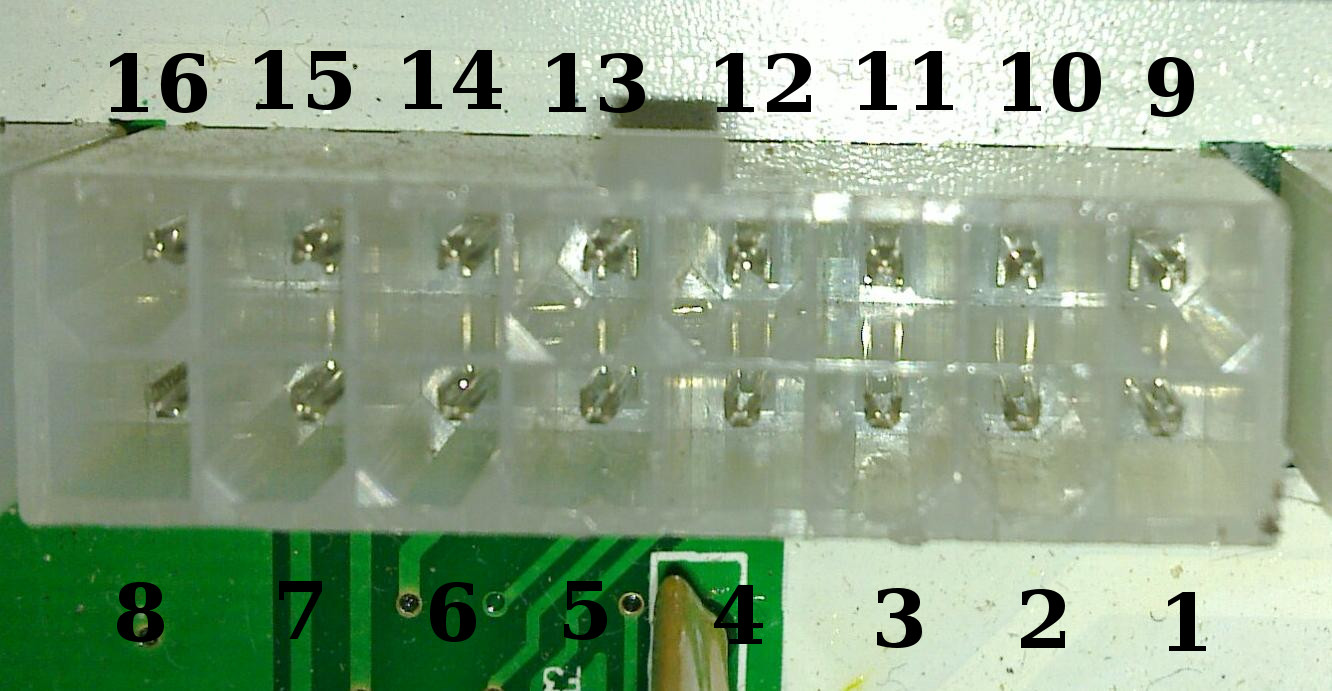
\includegraphics[width=3in]{images/16pin.jpg}
		\caption{Controller 16 pin output}
	\end{figure}
}

\frame {
	\frametitle{Signal Identification and Measurement System}
	
	\begin{figure}
		\centering
		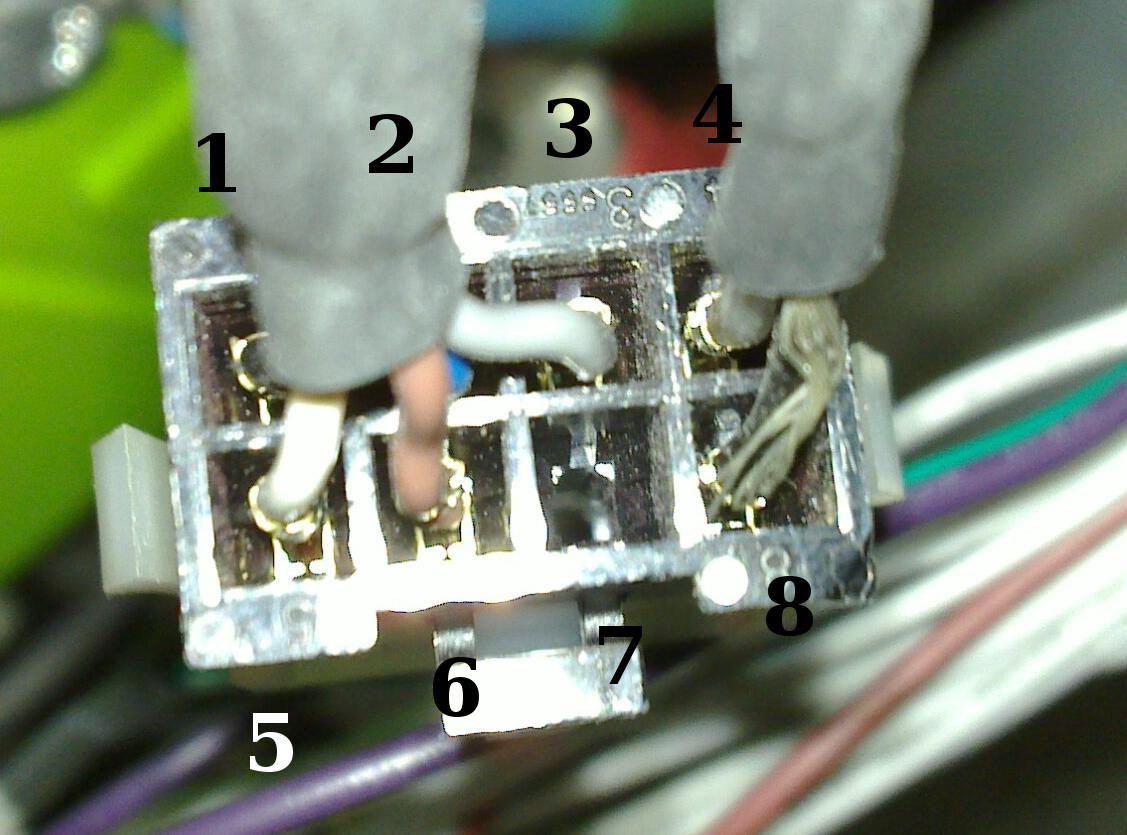
\includegraphics[width=3in]{images/hall.jpg}
		\caption{8 pin hall effect sensors input/output}
	\end{figure}
}

\subsection{Vehicle Simulation}

\frame {
	\frametitle{Why Vehicle Simulation?}
	
	\begin{itemize}
		\item Baseline data
		\item Strategies creation tool
		\item Study effect of a component
		\item Proprietary electric motor and controller
	\end{itemize}
}

\frame {
	\frametitle{Components}
	
	\begin{itemize}
		\item Track
		\item Electric Motor
		\item Vehicle Dynamics
	\end{itemize}
}

\frame {
	\frametitle{Sepang North Track}
	
	\begin{figure}
		\centering
		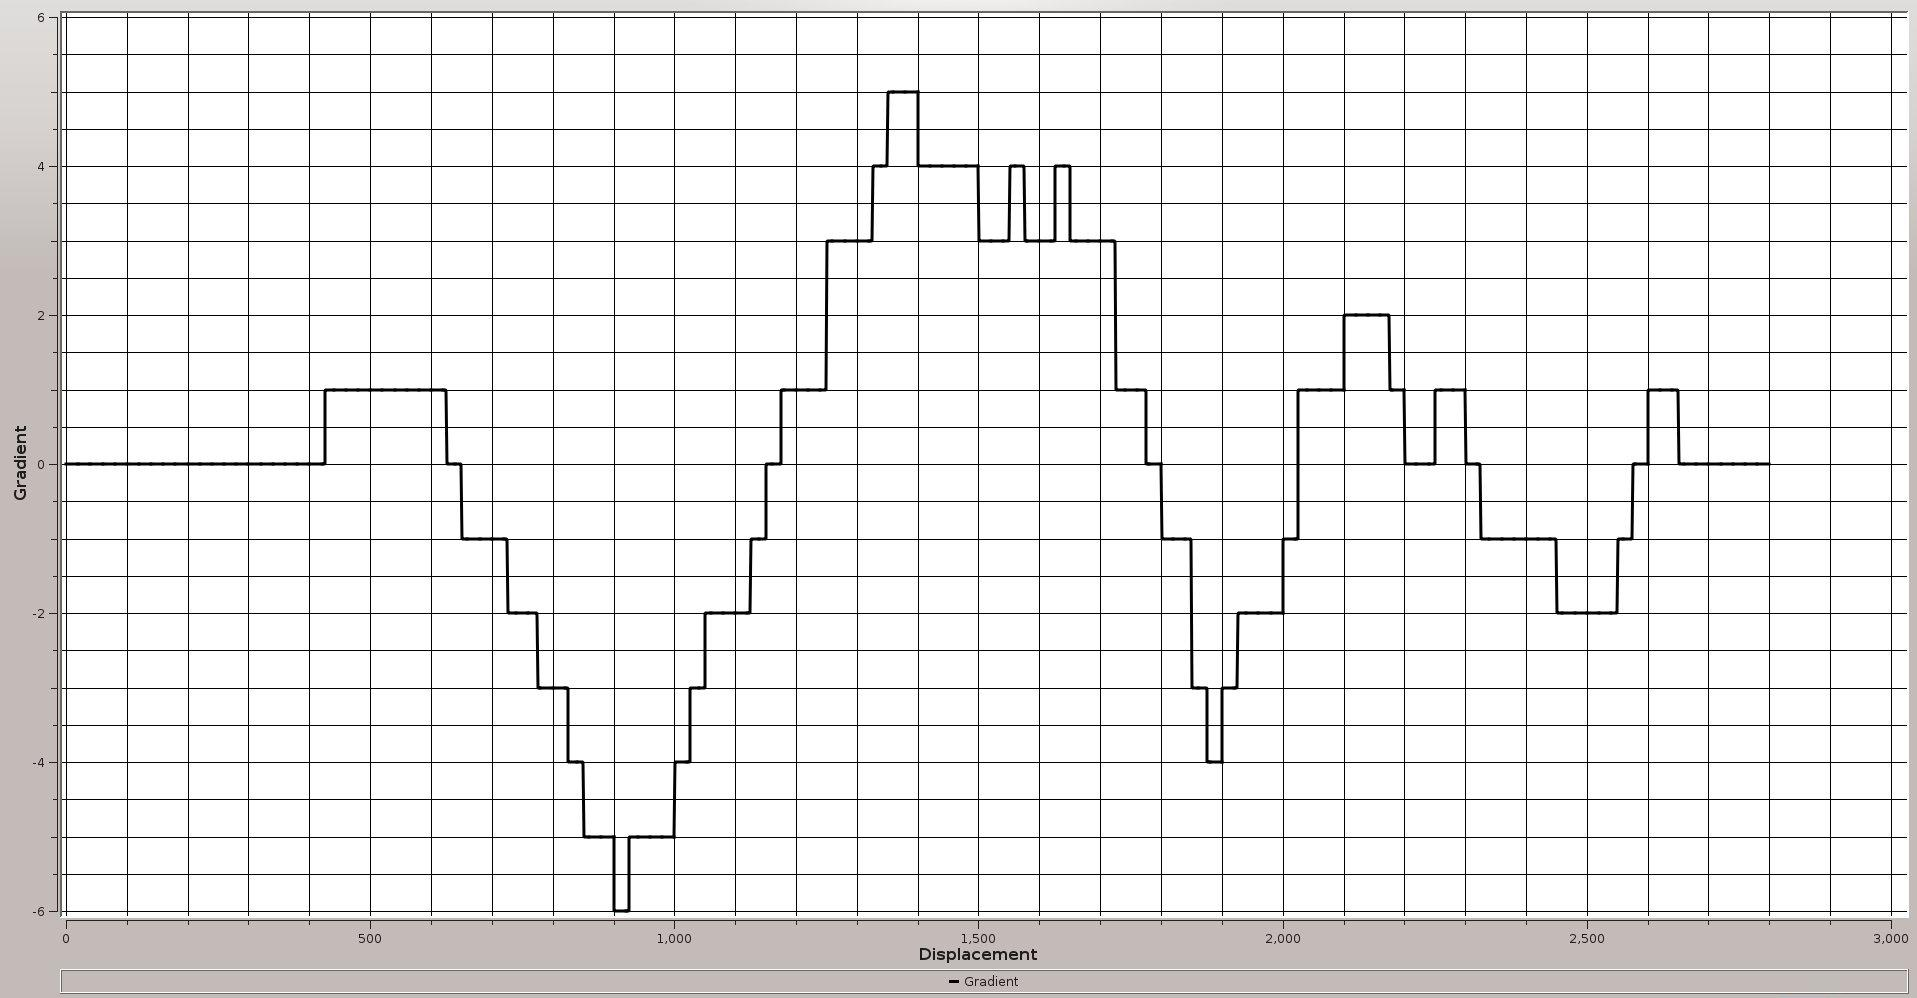
\includegraphics[width=4in]{images/track_gradient.jpg}
		\caption{Sepang North Track gradient graph}
	\end{figure}
}

\frame {
	\frametitle{Electric Motor}
	
	\begin{figure}
		\centering
		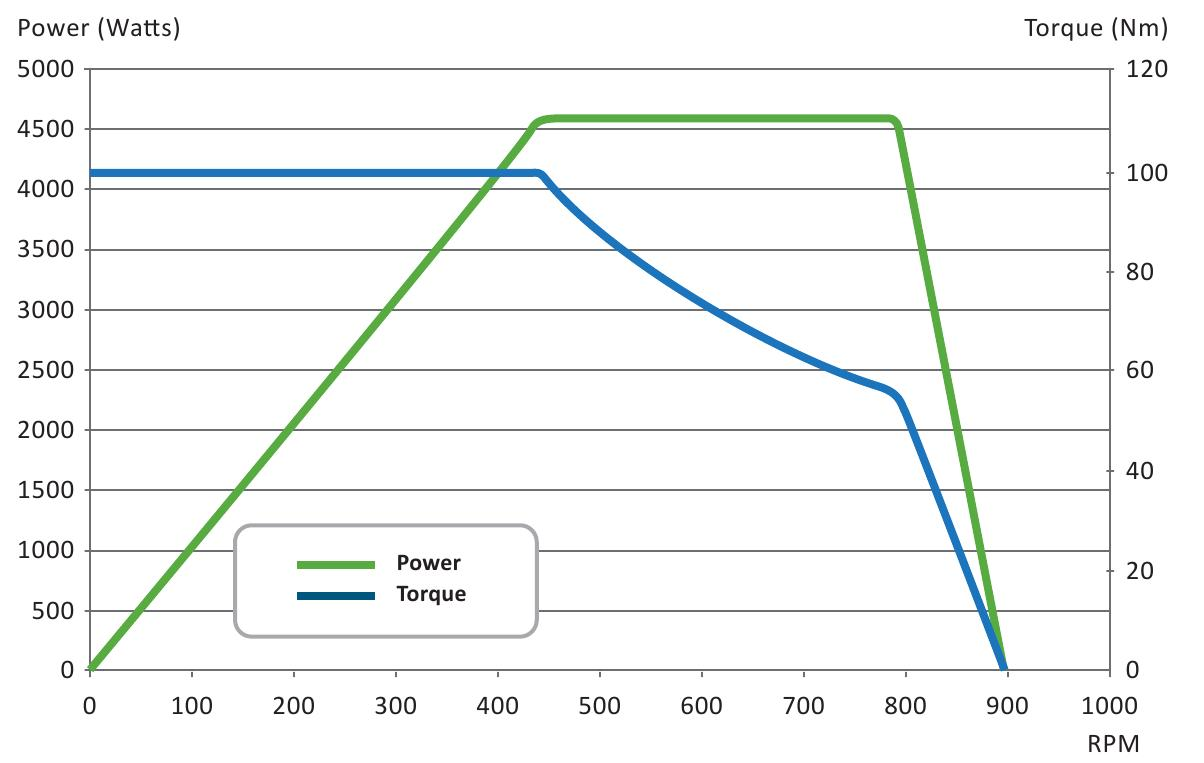
\includegraphics[width=3in]{images/kld_motor_torque_curve.jpg}
		\caption{Torque and power output curve of KLD D1064R, source: KLD}
	\end{figure}
}

\frame {
	\frametitle{Electric Motor}
	
	\begin{equation}
	T = \begin{cases} 100 N.m, & \mbox{for (0 - 440 RPM)} \\ [0.0003(RPM)^2 - 0.493(RPM) + 260] N.m, & \mbox{for (441 - 800 RPM)} \\ [-0.56(RPM) + 504] N.m, & \mbox{for (801 - 900 RPM)} \end{cases}
	\end{equation}

}

\frame {
	\frametitle{Vehicle Dynamics}
	
	\begin{itemize}
		\item Air drag
		\begin{equation}
			F_{drag} = \frac{1}{2}\rho C_{d} A v^2
		\end{equation}
		\item Rolling resistance
		\begin{equation}
			F_{roll} = mg C_{rr}
		\end{equation}
		\item Uphill/Downhill
		\begin{equation}
			F_{slope} = mgsin\theta
		\end{equation}
	\end{itemize}
}

\frame {
	\frametitle{Vehicle Dynamics}
	
	\begin{itemize}
		\item Combined
		\begin{equation}
			\sum F_{resistance} = mgsin\theta + mg C_{rr} + \frac{1}{2}\rho C_{d} A v^2 
		\end{equation}
		\item Vehicle acceleration
		\begin{equation}
			a = \frac{(\frac{\tau}{R} - \sum F_{resistance})}{m}
		\end{equation}
	\end{itemize}
}

\section{Result}
\subsection {Signal Identification and Measurement System}
\frame{
	\frametitle{Speed Signal}
	\scriptsize
	\begin{table}[htbp]
	\begin{center}
	\begin{tabular}{|c|c|c|}
	\hline
	\textbf{Voltage Probe} & \textbf{Ground Probe} & \textbf{Voltage} \\ \hline
	2 & 1 & -56.6 \\ \hline
	3 & 1 & -44.2 \\ \hline
	4 & 1 & 0.0 \\ \hline
	5 & 1 & -55.9 \\ \hline
	6 & 1 & -56.6 \\ \hline
	7 & 1 & 0.0 \\ \hline
	8 & 1 & 0.0 \\ \hline
	9 & 1 & -33.4 \\ \hline
	10 & 1 & -33.4 \\ \hline
	11 & 1 & -56.6 \\ \hline
	12 & 1 & -28.3 \\ \hline
	13 & 1 & -24.0 \\ \hline
	14 & 1 & -23.3 \\ \hline
	15 & 1 & -21.1 \\ \hline
	16 & 1 & -23.7 \\ \hline
	\end{tabular}
	\end{center}
	\caption{Result of signal tapping with the ground probe on pin 1 and voltage terminal on pin 2 to pin 16.}
	\label{tb:speedIdenGnd1}
	\end{table}
}

\frame {
	\frametitle{Speed Signal}
	\scriptsize
	\begin{table}[htbp]
	\begin{center}
	\begin{tabular}{|c|c|c|}
	\hline
	\textbf{Voltage Probe} & \textbf{Ground Probe} & \textbf{Voltage} \\ \hline
	1 & 2 & 56.8 \\ \hline
	3 & 2 & 12.4 \\ \hline
	4 & 2 & 0.0 \\ \hline
	5 & 2 & 0.0 \\ \hline
	6 & 2 & 0.0 \\ \hline
	7 & 2 & 0.0 \\ \hline
	8 & 2 & 0.0 \\ \hline
	9 & 2 & 22.6 \\ \hline
	10 & 2 & 22.6 \\ \hline
	11 & 2 & 0.0 \\ \hline
	12 & 2 & 29.9 \\ \hline
	13 & 2 & 0.0 \\ \hline
	14 & 2 & 0.0 \\ \hline
	15 & 2 & 0.0 \\ \hline
	16 & 2 & 0.0 \\ \hline
	\end{tabular}
	\end{center}
	\caption{Result of signal tapping with the ground probe on pin 2 and voltage terminal on pin 1, pin 3 to pin 16.}
	\label{tb:speedIdenGnd2}
	\end{table}
}

\frame {
	\frametitle{Speed Signal}
	\scriptsize
	\begin{table}[htbp]
	\begin{center}
	\begin{tabular}{|c|c|c|}
	\hline
	\textbf{Voltage Probe} & \textbf{Ground Probe} & \textbf{Voltage} \\ \hline
	1 & 2 & 56.7 \\ \hline
	3 & 2 & 12.4 \\ \hline
	4 & 2 & 0.0 \\ \hline
	5 & 2 & -3.4 \\ \hline
	6 & 2 & 0.0 \\ \hline
	7 & 2 & 0.7-2.4 \\ \hline
	8 & 2 & 0.7-3.2 \\ \hline
	9 & 2 & 22.6 \\ \hline
	10 & 2 & 22.6 \\ \hline
	11 & 2 & 0.0 \\ \hline
	12 & 2 & 27.8 \\ \hline
	13 & 2 & 0.0 \\ \hline
	14 & 2 & 0.0 \\ \hline
	15 & 2 & 0.0 \\ \hline
	16 & 2 & 0.0 \\ \hline
	\end{tabular}
	\end{center}
	\caption{Result of signal tapping with the ground probe on pin 2 and voltage terminal on pin 1, pin 3 to pin 16 and the motor rotating.}
	\label{tb:speedIdenGnd2Running}
	\end{table}
}

\frame {
	\frametitle{Speed Signal}
	\begin{itemize}
		\item Pin 1: Battery voltage
		\item Pin 2, 6, 11: Ground
		\item Pin 3: 12V power supply
		\item Pin 5: Speed output signal
	\end{itemize}
}

\frame {
	\frametitle{Hall Effect Sensors Signal}
	\scriptsize
	\begin{table}[htbp]
	\begin{center}
	\begin{tabular}{|c|c|c|}
	\hline
	\textbf{Voltage Probe} & \textbf{Ground Probe} & \textbf{Voltage} \\ \hline
	1 & 8 & 10.4 \\ \hline
	2 & 8 & 10.4 \\ \hline
	3 & 8 & 10.4 \\ \hline
	4 & 8 & 3.1 \\ \hline
	5 & 8 & 0.2 \\ \hline
	6 & 8 & 0.1 \\ \hline
	\end{tabular}
	\end{center}
	\caption{Result of hall effect sensors signal tapping with the ground probe on pin 8 and voltage terminal on pin 1 to pin 6.}
	\label{tb:hallIdenGnd8}
	\end{table}
}

\frame {
	\frametitle{Hall Effect Sensors Signal}
	\begin{itemize}
		\item Pin 2, 3, 5: Hall Effect Sensors output
		\item Pin 1: Power Supply
		\item Pin 8: Ground
	\end{itemize}
}

\frame {
	\frametitle{Measurement System}
	\begin{figure}
		\centering
		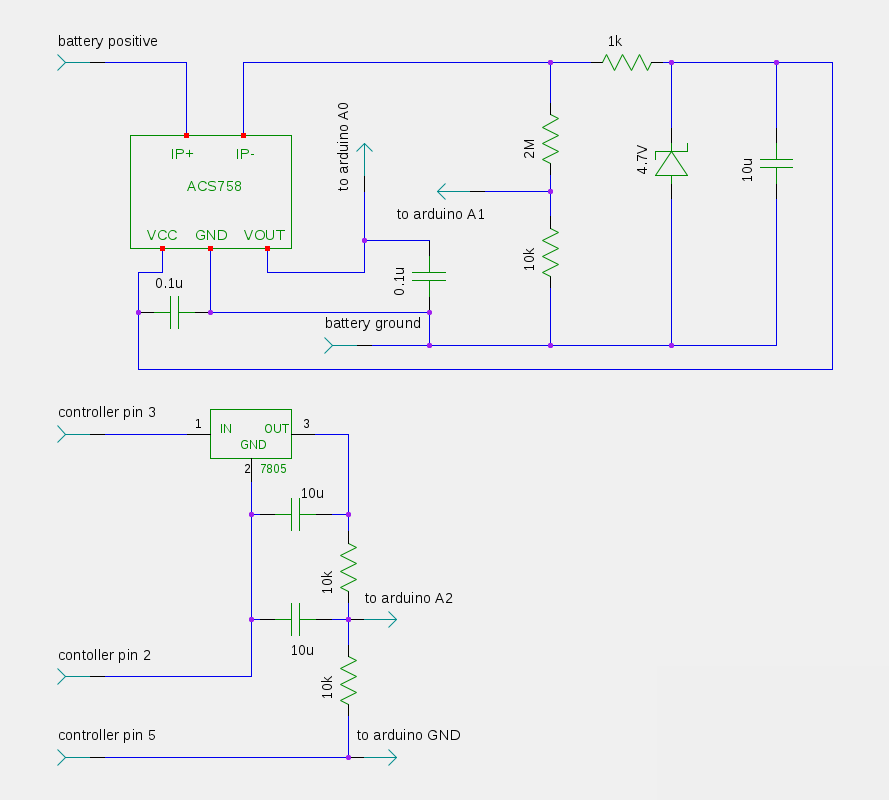
\includegraphics[width=3in]{images/sch.png}
		\caption{Schematic of the Measurement System}
	\end{figure}
}

\frame {
	\frametitle{Measurement System}
	\begin{figure}
		\centering
		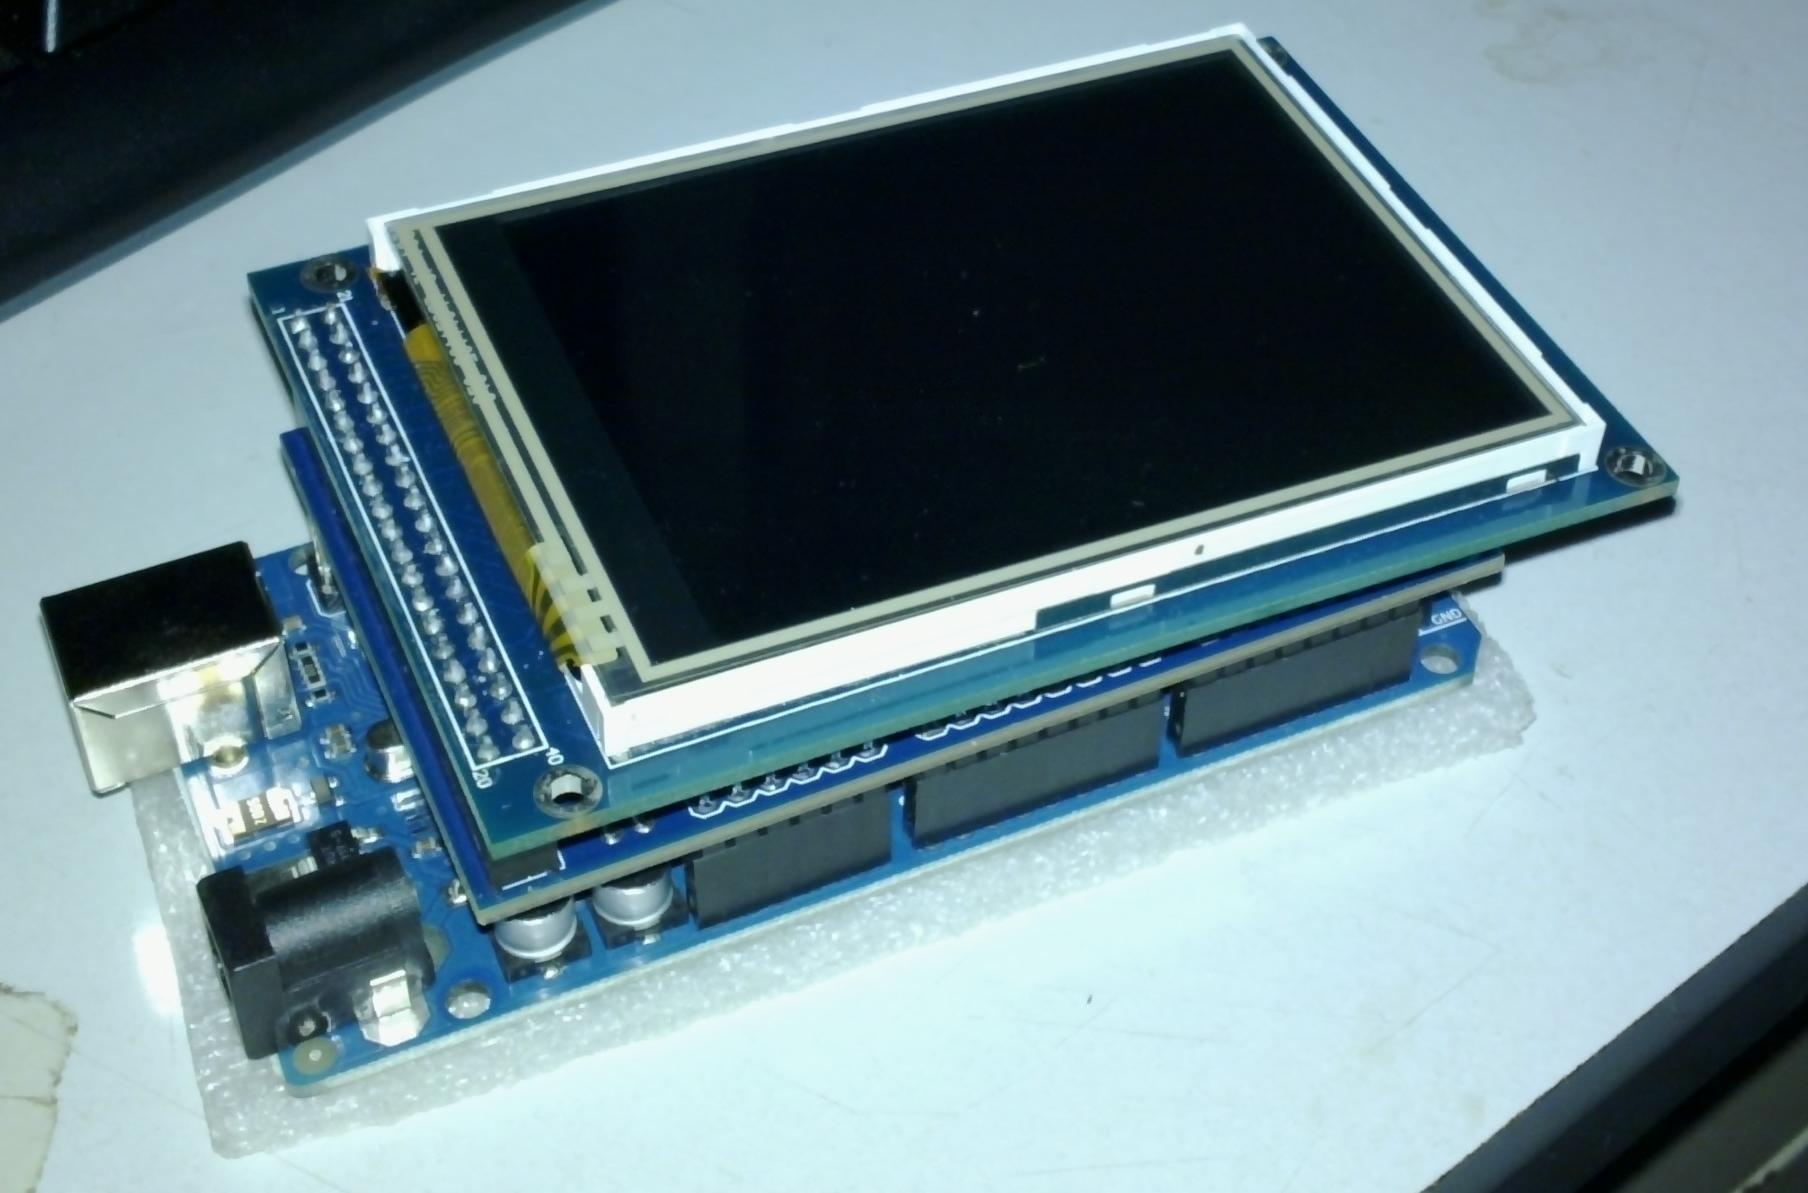
\includegraphics[width=3in]{images/arduino.jpg}
		\caption{Arduino Microcontroller, display shield and LCD display}
	\end{figure}
}

\subsection {Vehicle Simulation}

\frame {
	\frametitle{Vehicle Simulation}
	\begin{figure}[htb]
	\centering
	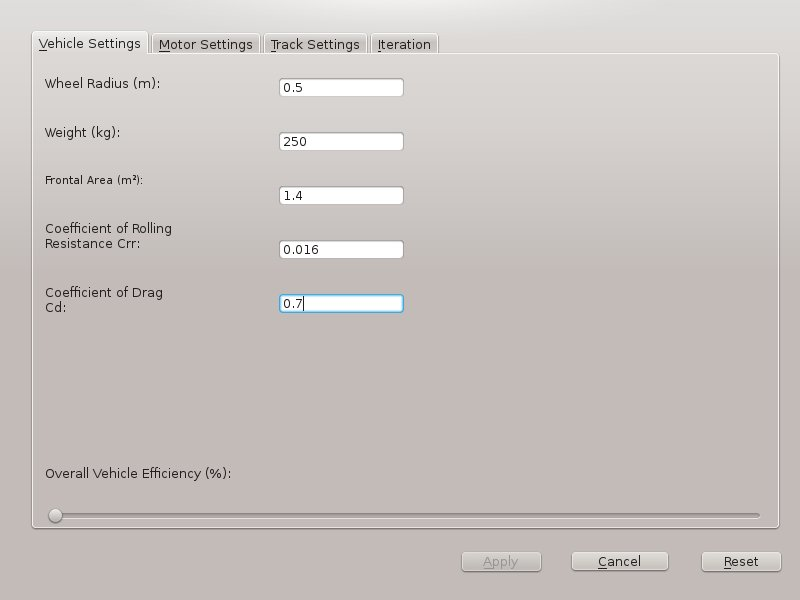
\includegraphics[width=3in]{images/vehicle_settings.jpg}
	\caption{Vehicle parameter for initializing the vehicle model}
	\label{im:vehicleSettings}
	\end{figure}
}

\frame {
	\frametitle{Vehicle Simulation}
	\begin{figure}[htb]
	\centering
	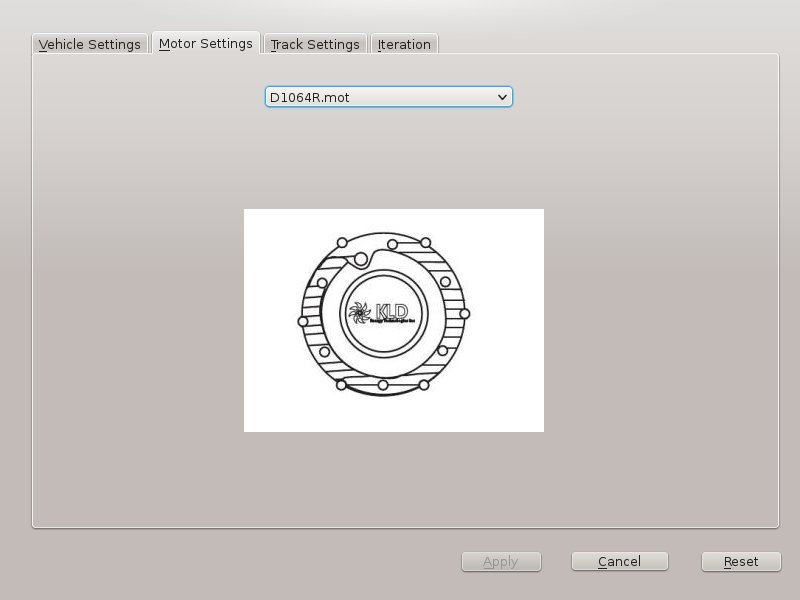
\includegraphics[width=3in]{images/motor_settings.jpg}
	\caption{Choosing the motor model}
	\label{im:motorSettings}
	\end{figure}
	
}

\frame {
	\frametitle{Vehicle Simulation}
	\begin{figure}[htb]
	\centering
	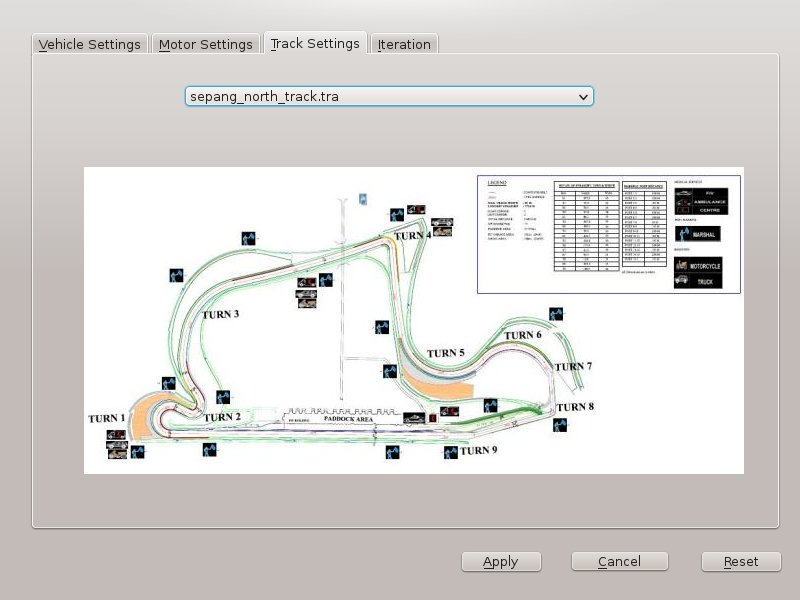
\includegraphics[width=3in]{images/track_settings.jpg}
	\caption{Choosing the track model}
	\label{im:trackSettings}
	\end{figure}
}

\frame {
	\frametitle{Vehicle Simulation}
	\begin{figure}[htb]
	\centering
	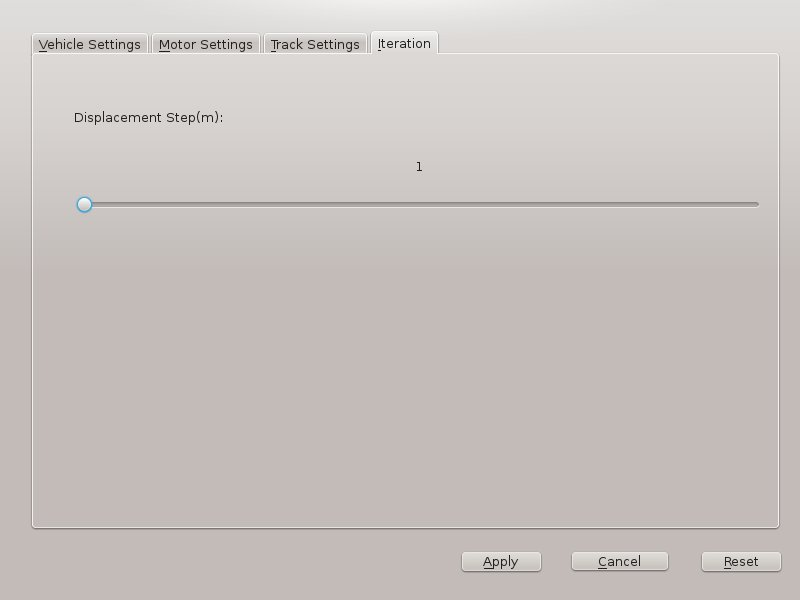
\includegraphics[width=3in]{images/iteration_step.jpg}
	\caption{Setting the displacement interval for iteration}
	\label{im:iterationStep}
	\end{figure}
}

\frame {
	\frametitle{Vehicle Simulation}
	\scriptsize
	\begin{table}[htbp]
	\begin{center}
	\begin{tabular}{|c|c|}
	\hline
	\textbf{Parameter} & \textbf{Value} \\ \hline
	Wheel Radius & 0.5 m \\ \hline
	Total Vehicle Mass & 250 kg \\ \hline
	Frontal Area & 1.4 $m^2$ \\ \hline
	Crr & 0.016 \\ \hline
	Cd & 0.7 \\ \hline
	\end{tabular}
	\end{center}
	\caption{Parameters for building the electric vehicle model}
	\label{tb:vehicleModelParameter}
	\end{table}
}

\subsection {Strategies}

\frame {
	\frametitle{Strategies}
	\begin{enumerate}
		\item Full Throttle Everywhere
		\item Preset Strategy 1
		\item Preset Strategy 2
		\item Preset Strategy 3
	\end{enumerate}
}

\frame {
	\frametitle{Full Throttle Everywhere}
	\begin{figure}[htb]
	\centering
	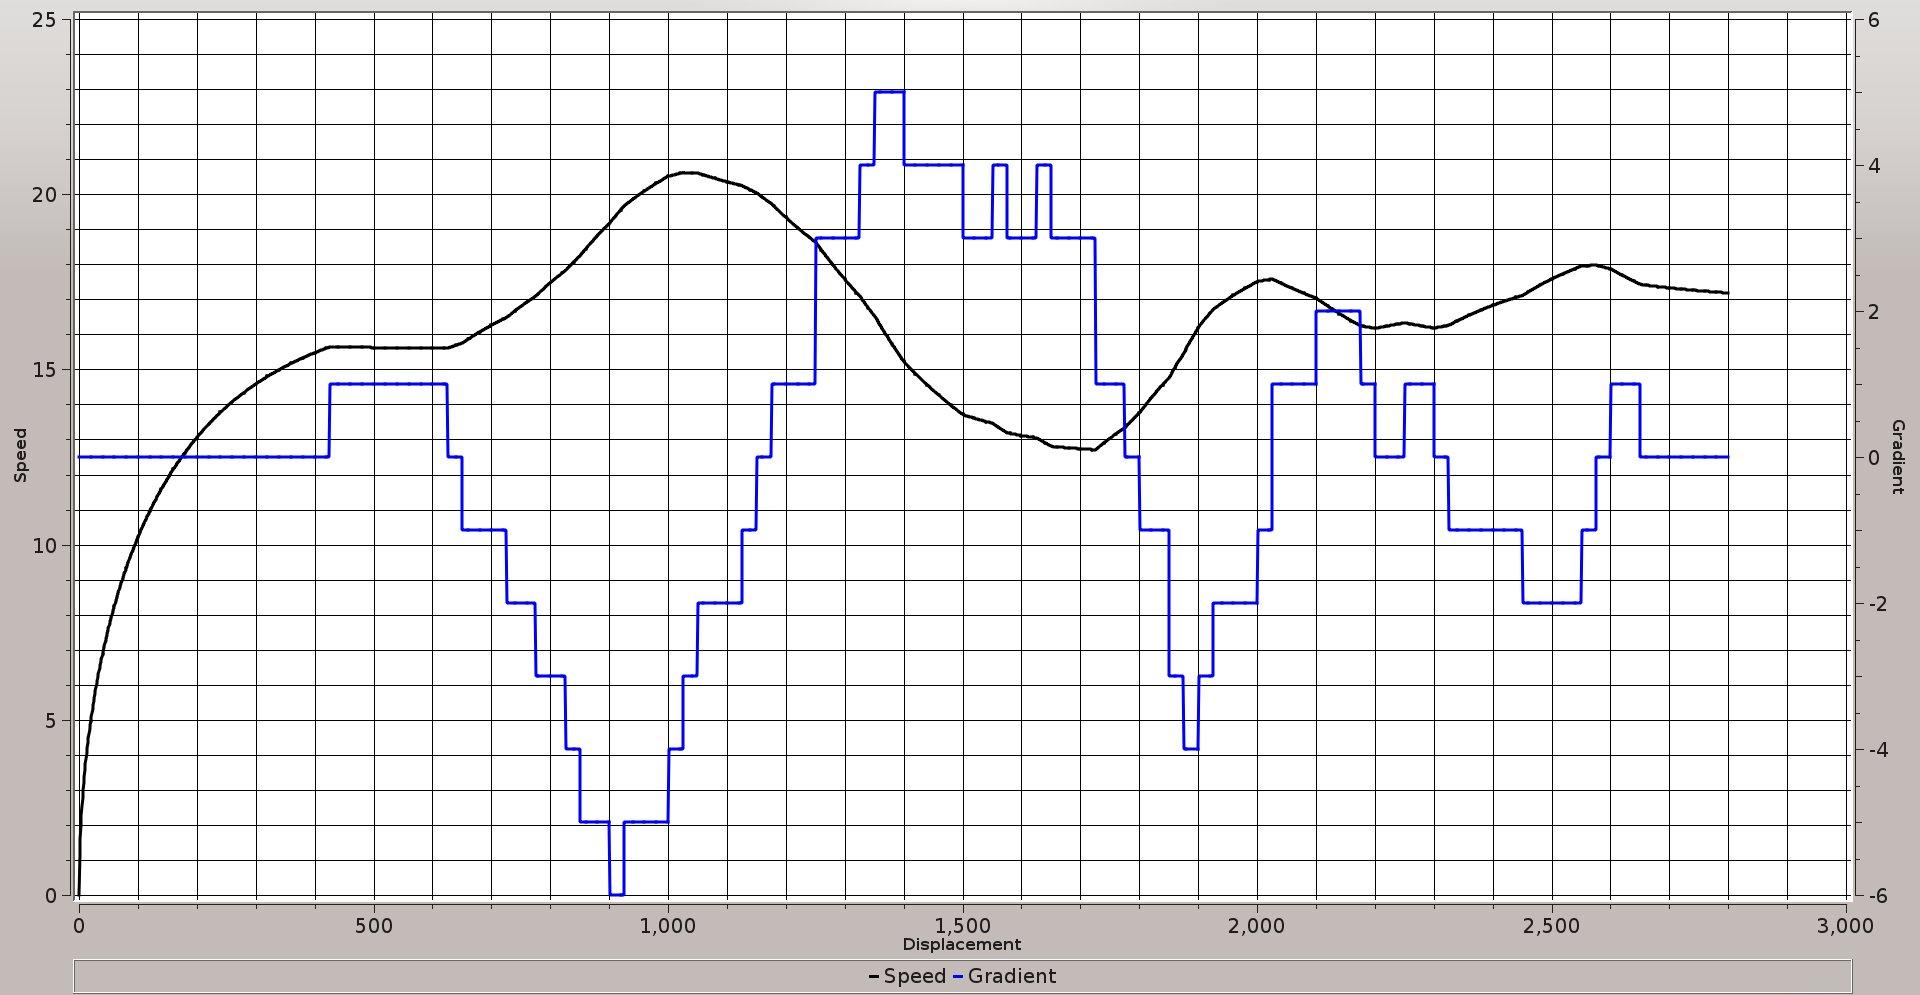
\includegraphics[width=3in]{images/0_1.jpg}
	\caption{Graph of speed and gradient versus displacement for "full throttle everywhere"}
	\end{figure}
}

\frame {
	\frametitle{Full Throttle Everywhere}
	\begin{figure}[htb]
	\centering
	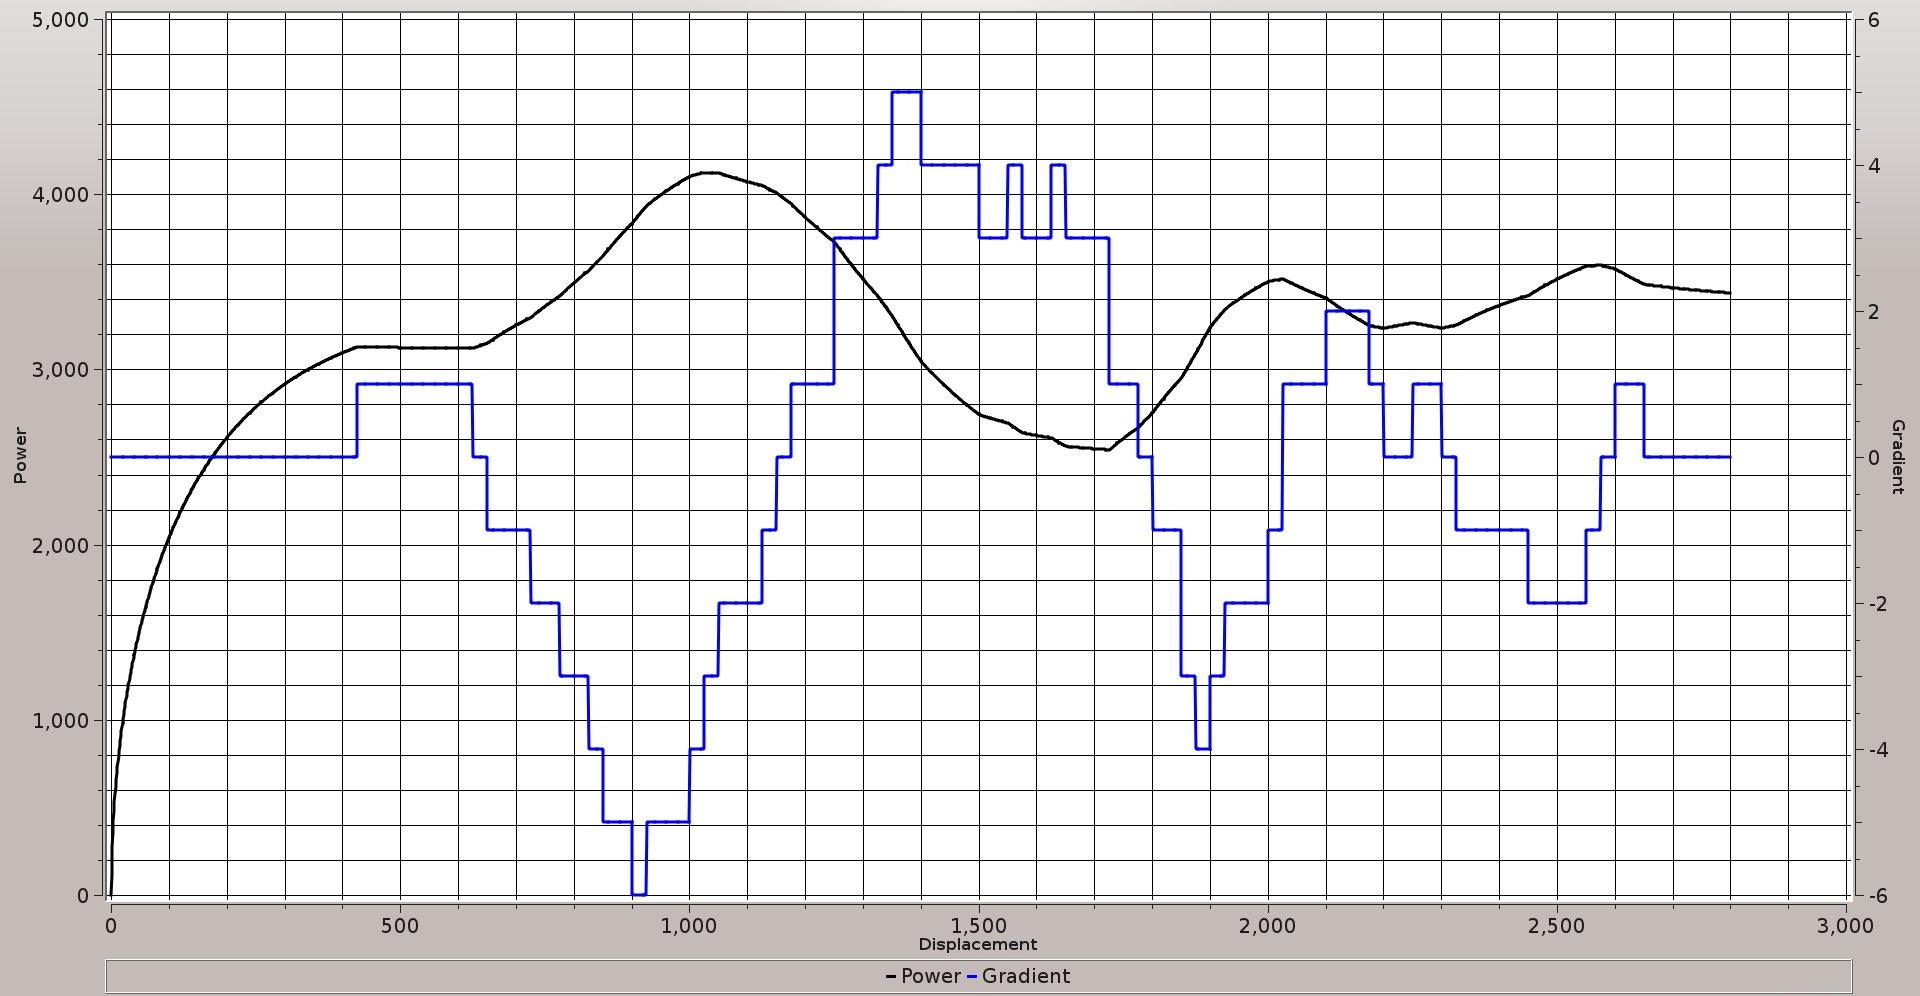
\includegraphics[width=3in]{images/0_2.jpg}
	\caption{Graph of power and gradient versus displacement for "full throttle everywhere"}
	\end{figure}
}

\frame {
	\frametitle{Preset Strategy 1}
	\begin{figure}[htb]
	\centering
	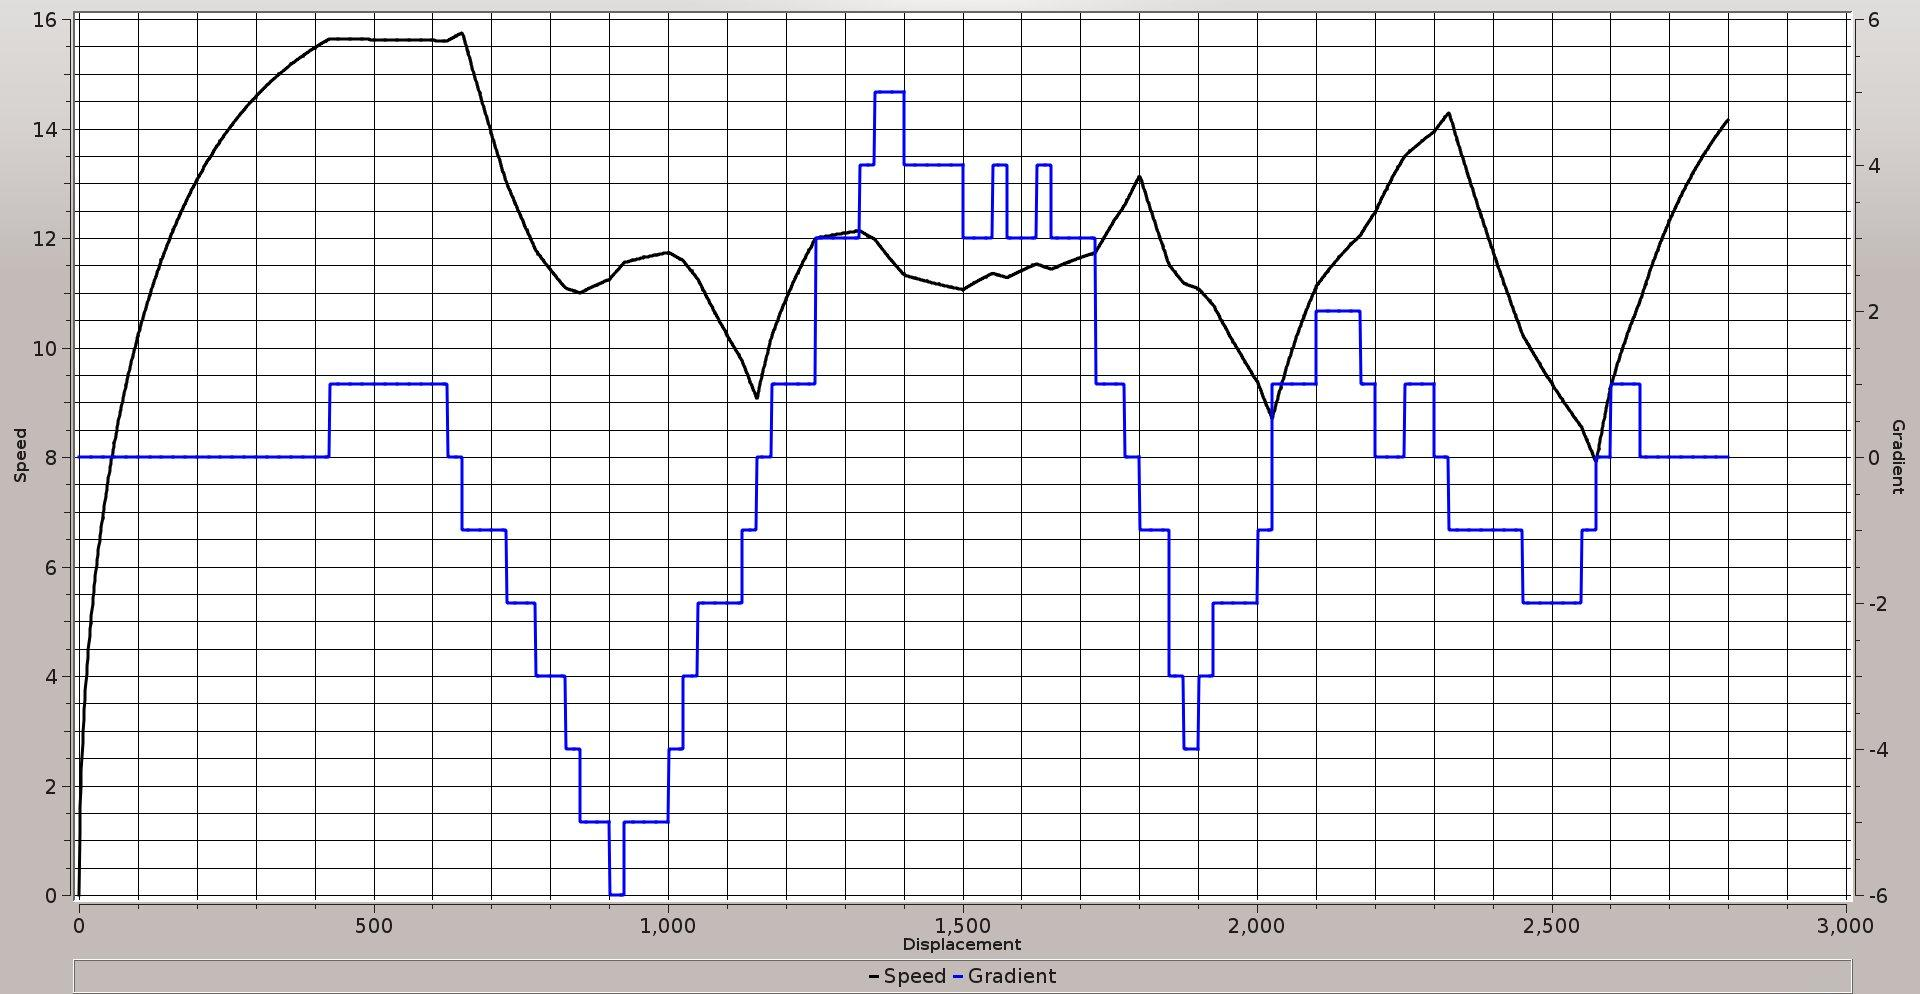
\includegraphics[width=3in]{images/1_1.jpg}
	\caption{Graph of Speed and Gradient versus displacement for "Preset Strategy 1"}
	\end{figure}
}

\frame {
	\frametitle{Preset Strategy 1}
	\begin{figure}[htb]
	\centering
	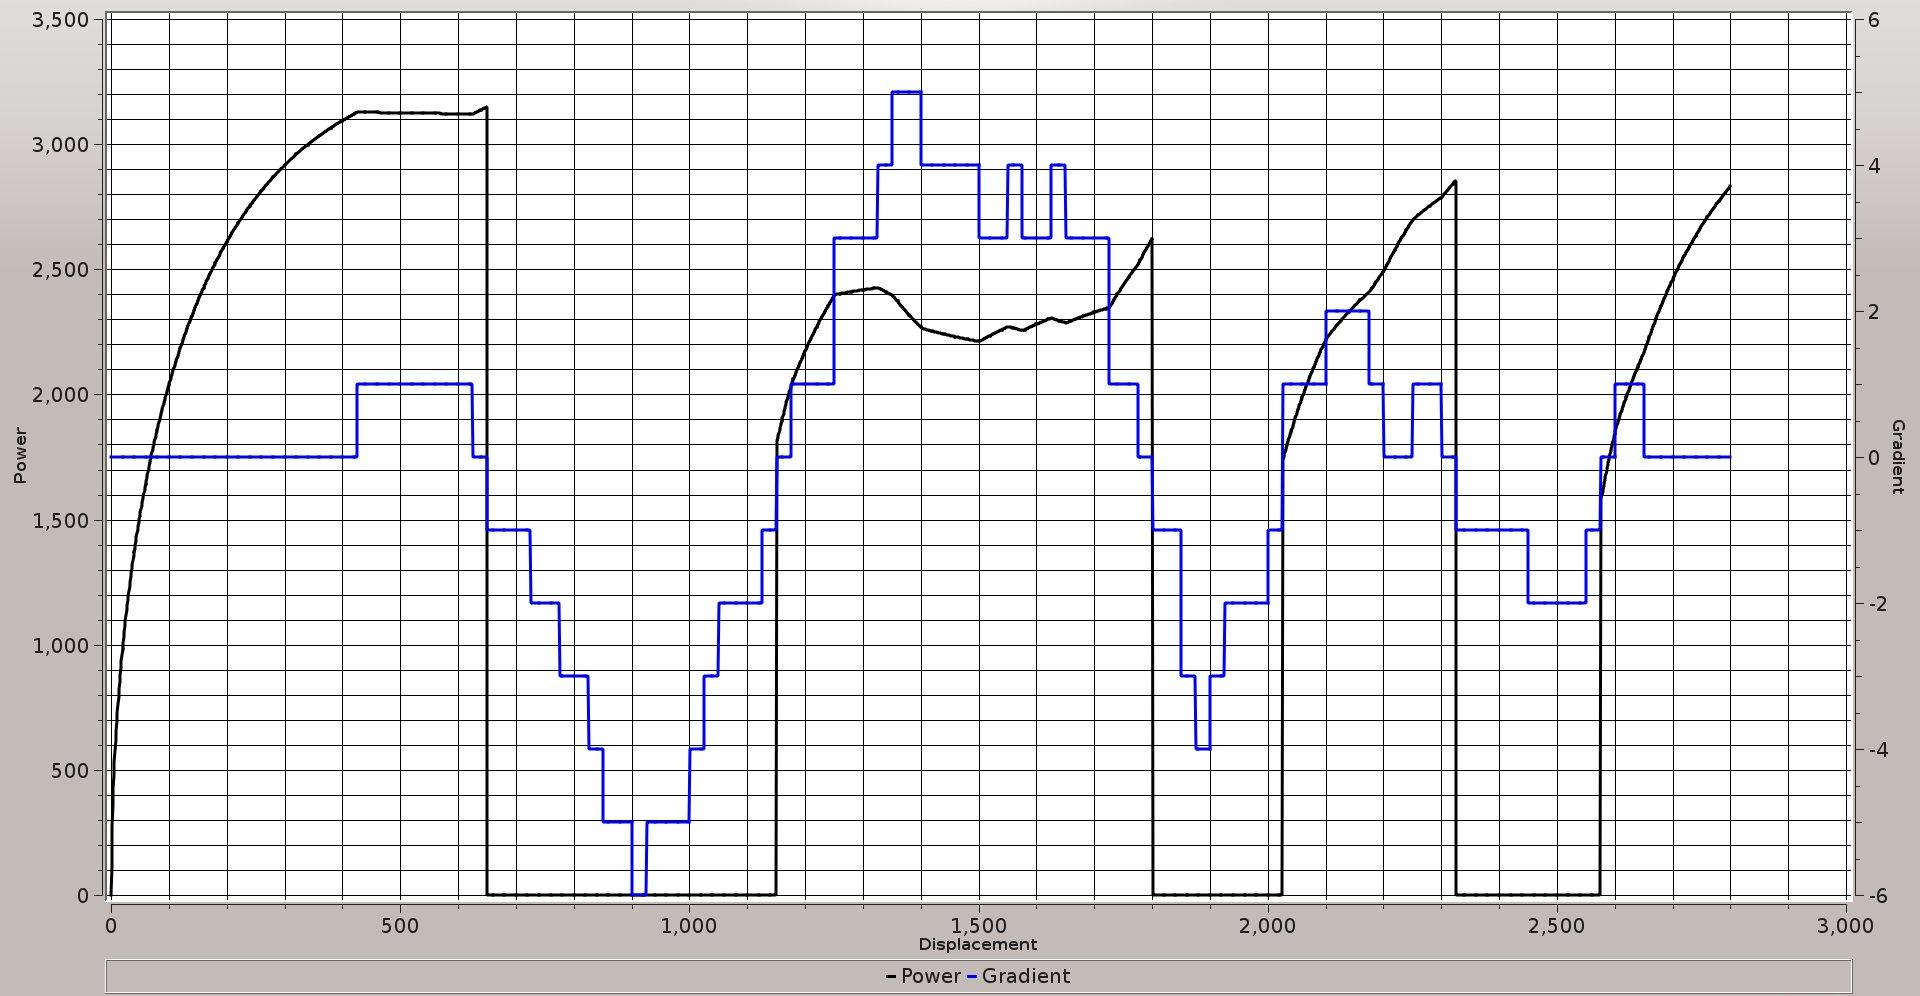
\includegraphics[width=3in]{images/1_2.jpg}
	\caption{Graph of Power and Gradient versus displacement for "Preset Strategy 1"}
	\end{figure}
}

\frame {
	\frametitle{Preset Strategy 2}
	\begin{figure}[htb]
	\centering
	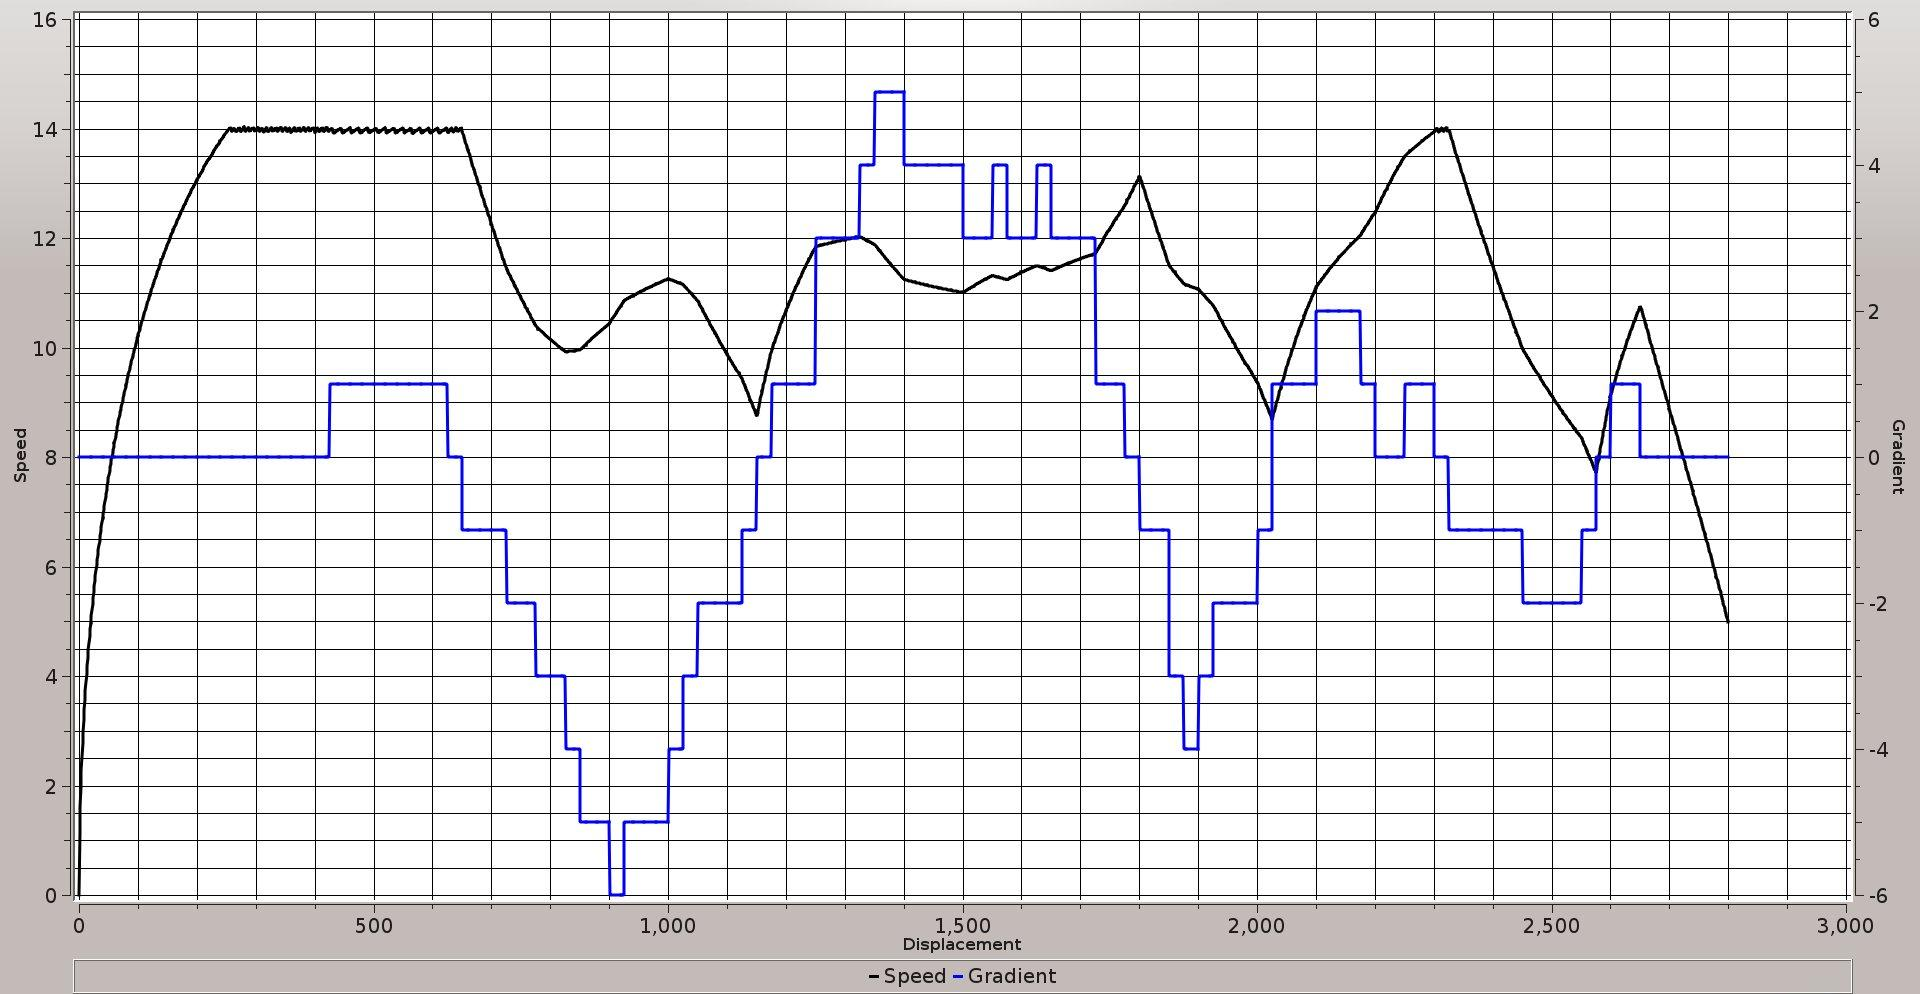
\includegraphics[width=3in]{images/2_1.jpg}
	\caption{Graph of Speed and Gradient versus displacement for "Preset Strategy 2"}
	\label{im:2_1}
	\end{figure}
}

\frame {
	\frametitle{Preset Strategy 2}
	\begin{figure}[htb]
	\centering
	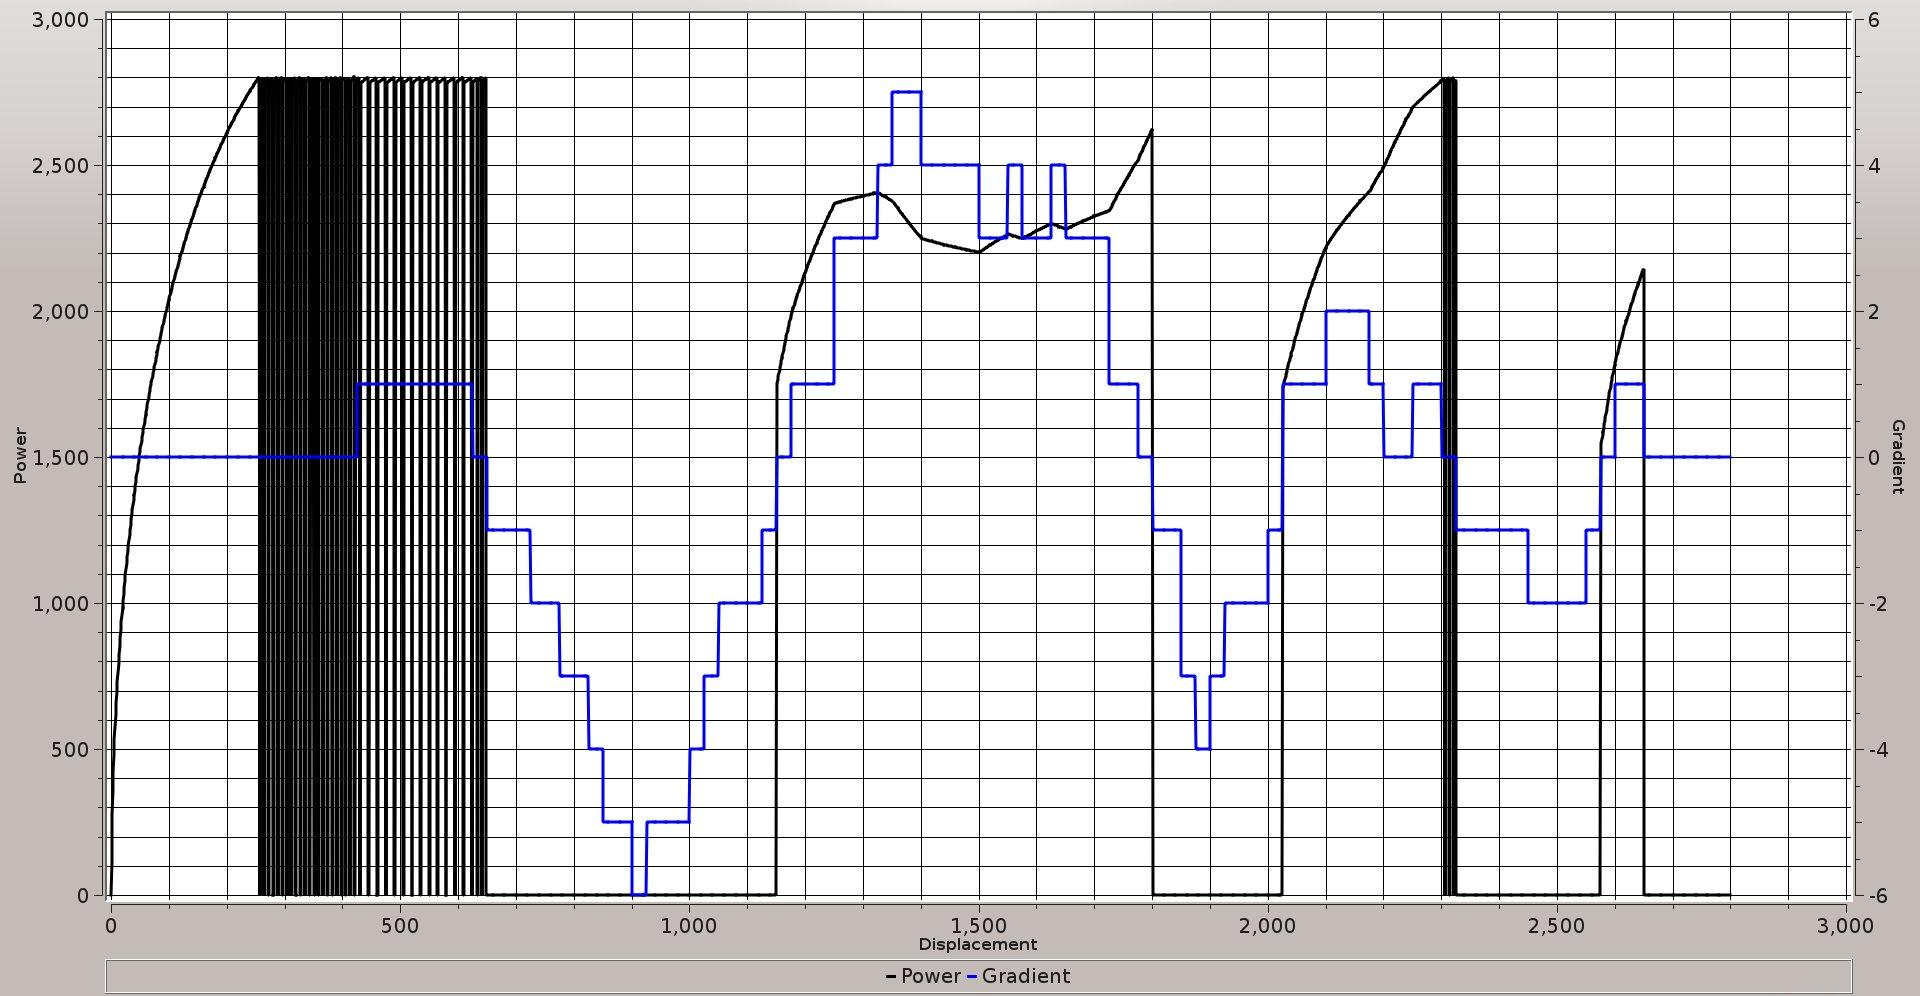
\includegraphics[width=3in]{images/2_2.jpg}
	\caption{Graph of Power and Gradient versus displacement for "Preset Strategy 2"}
	\label{im:2_2}
	\end{figure}
}

\frame {
	\frametitle{Preset Strategy 3}
	\begin{figure}[htb]
	\centering
	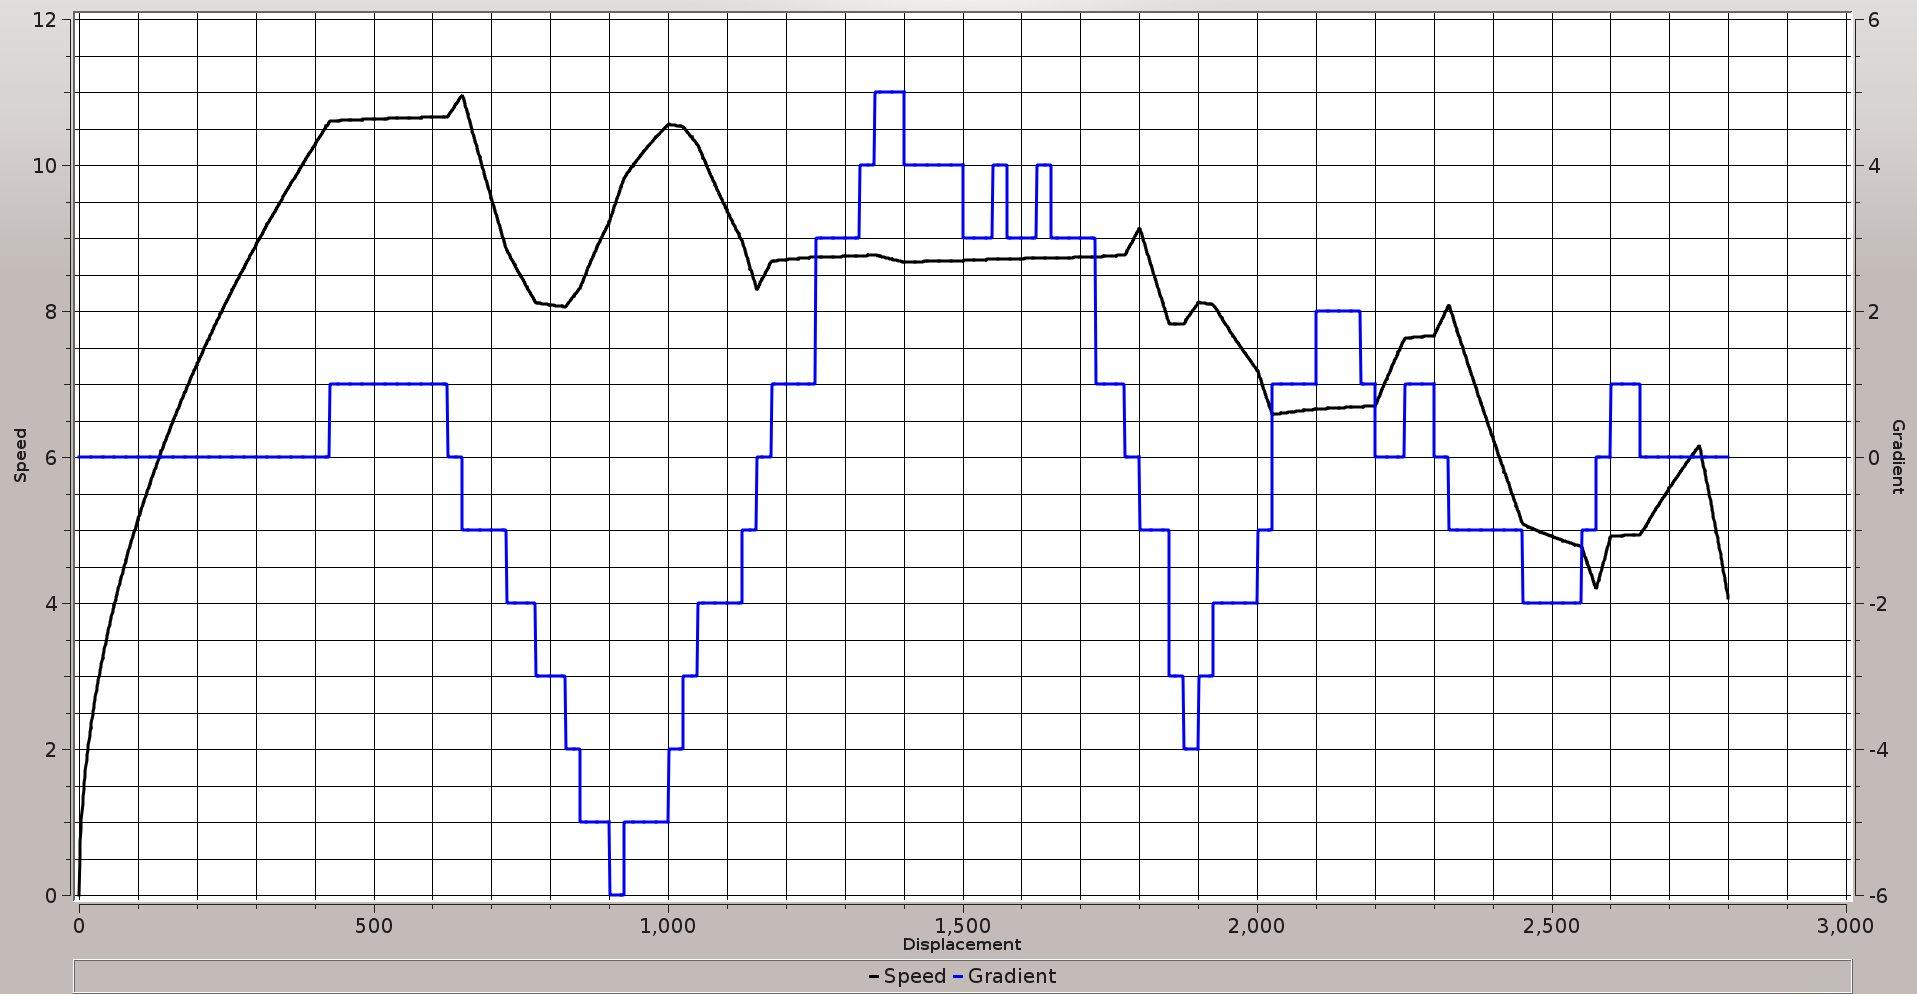
\includegraphics[width=3in]{images/3_1.jpg}
	\caption{Graph of Speed and Gradient versus displacement for "Preset Strategy 3"}
	\label{im:3_1}
	\end{figure}
}

\frame {
	\frametitle{Preset Strategy 3}
	\begin{figure}[htb]
	\centering
	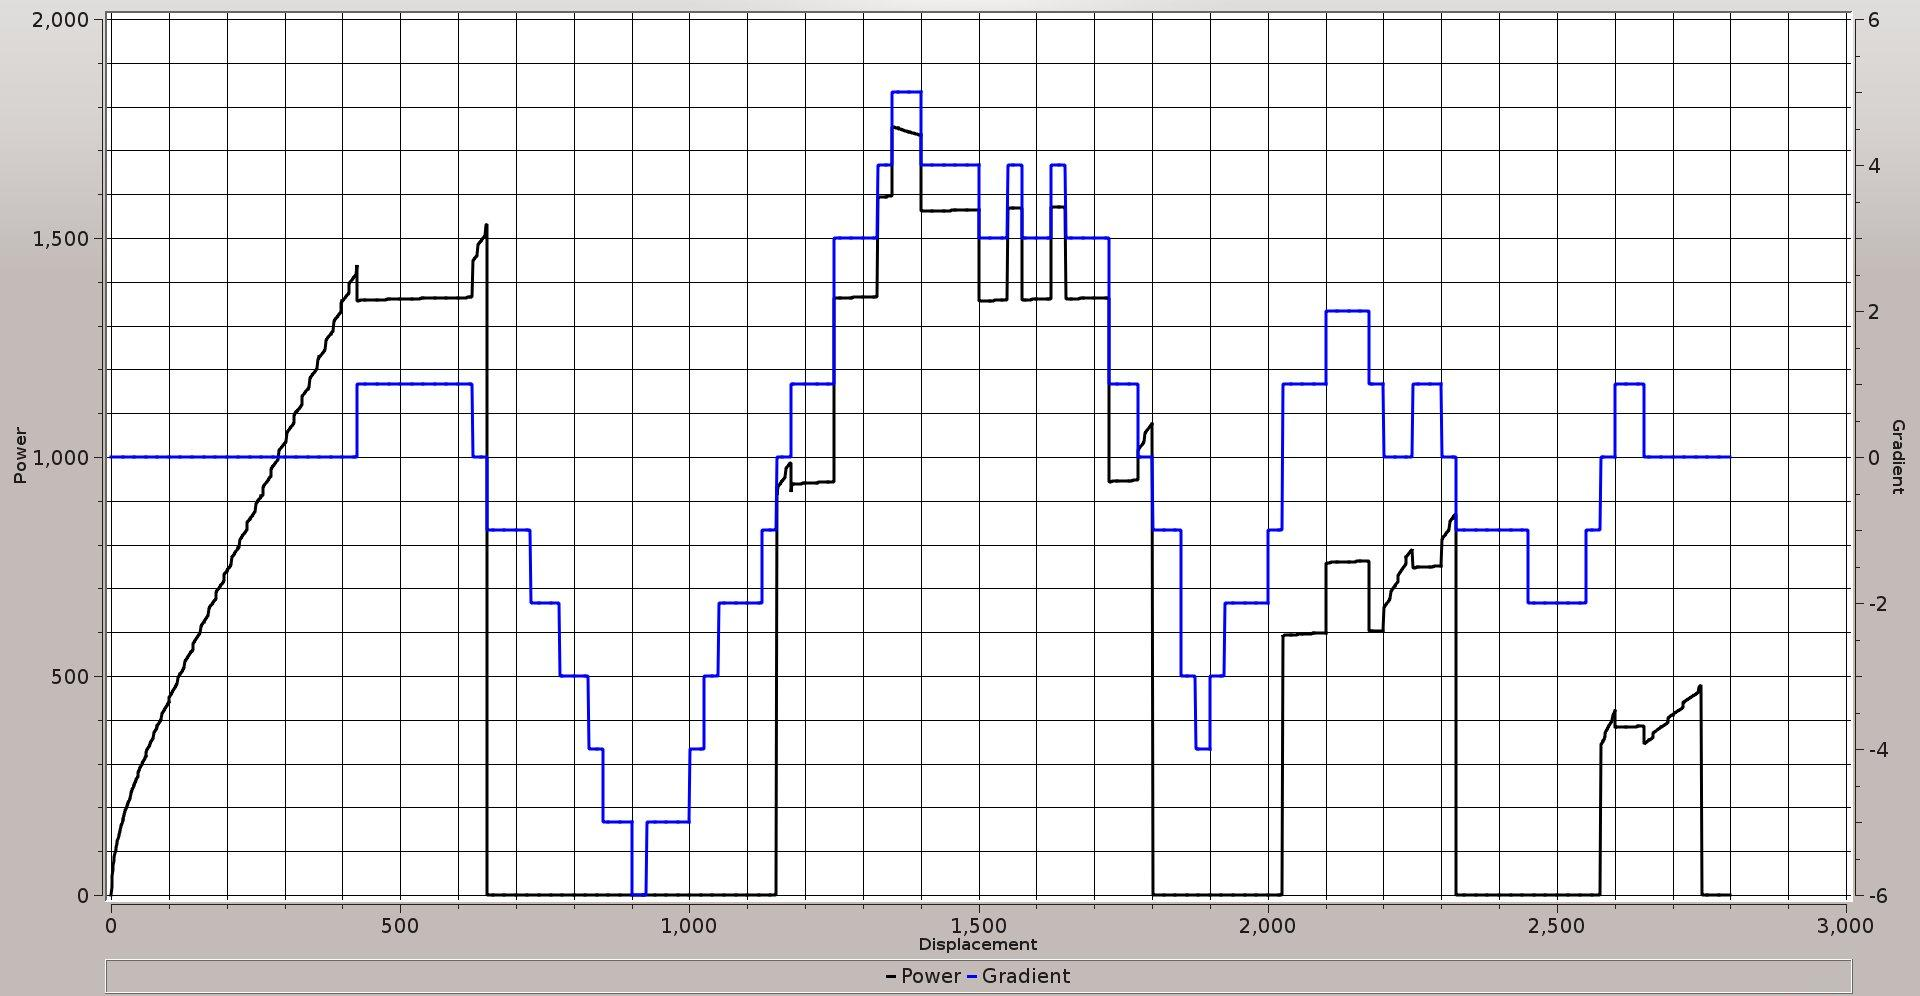
\includegraphics[width=3in]{images/3_2.jpg}
	\caption{Graph of Power and Gradient versus displacement for "Preset Strategy 3"}
	\label{im:3_2}
	\end{figure}
}

\frame {
	\frametitle{Comparison Between Strategies}
	\scriptsize
	\begin{table}[htbp]
	\begin{center}
	\begin{tabular}{|c|c|c|c|c|}
	\hline
	\textbf{Result} & \textbf{FTE} & \textbf{PS1} & \textbf{PS2} & \textbf{PS3} \\ \hline
	Total Energy Consumption & 560003J & 365004J & 318200J & 216385J \\ \hline
	Lap TIme & 186.981s & 246.554s & 261.699s & 390.491s \\ \hline
	Mileage & 18.0 km/kWh & 27.6 km/kWh & 31.7 km/kWh & 46.6 km/kWh \\ \hline
	\end{tabular}
	\end{center}
	\caption{Result comparison for various strategies}
	\end{table}
}

\frame {
	\frametitle{Comparison Between Strategies}
	\begin{figure}[htb]
	\centering
	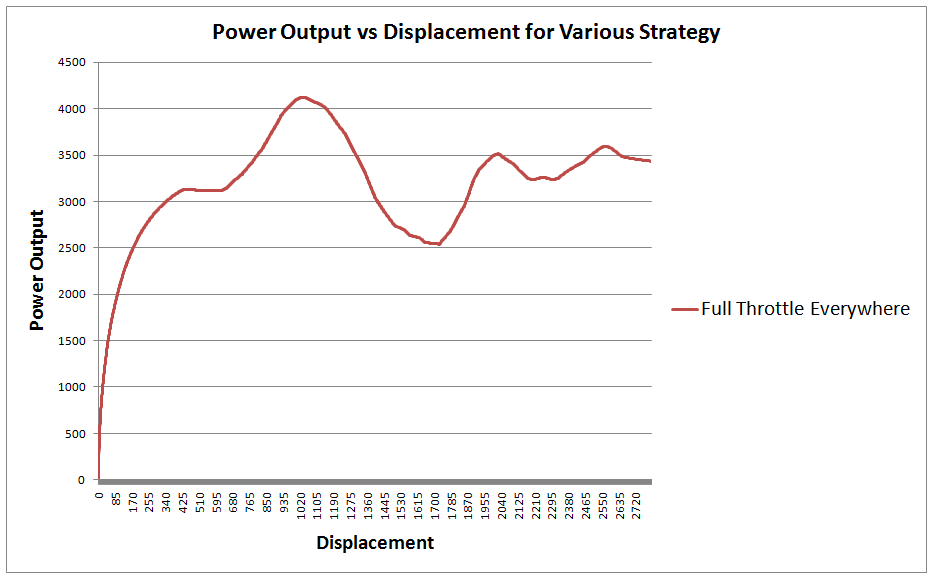
\includegraphics[width=4in]{images/power0.png}
	\caption{Graph of power output versus displacement for various strategy}
	\label{im:powerDisp}
	\end{figure}
}

\frame {
	\frametitle{Comparison Between Strategies}
	\begin{figure}[htb]
	\centering
	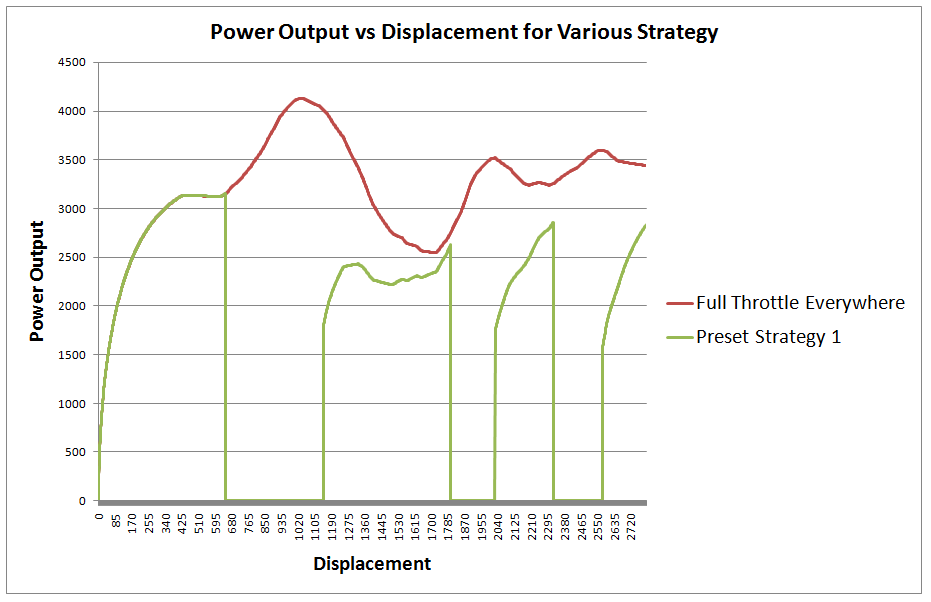
\includegraphics[width=4in]{images/power1.png}
	\caption{Graph of power output versus displacement for various strategy}
	\label{im:powerDisp}
	\end{figure}
}

\frame {
	\frametitle{Comparison Between Strategies}
	\begin{figure}[htb]
	\centering
	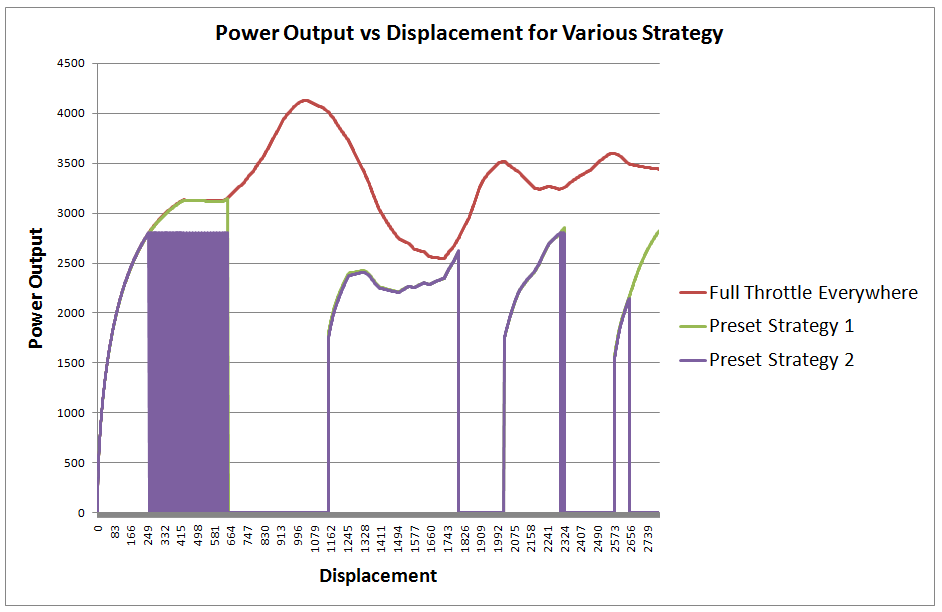
\includegraphics[width=4in]{images/power2.png}
	\caption{Graph of power output versus displacement for various strategy}
	\label{im:powerDisp}
	\end{figure}
}

\frame {
	\frametitle{Comparison Between Strategies}
	\begin{figure}[htb]
	\centering
	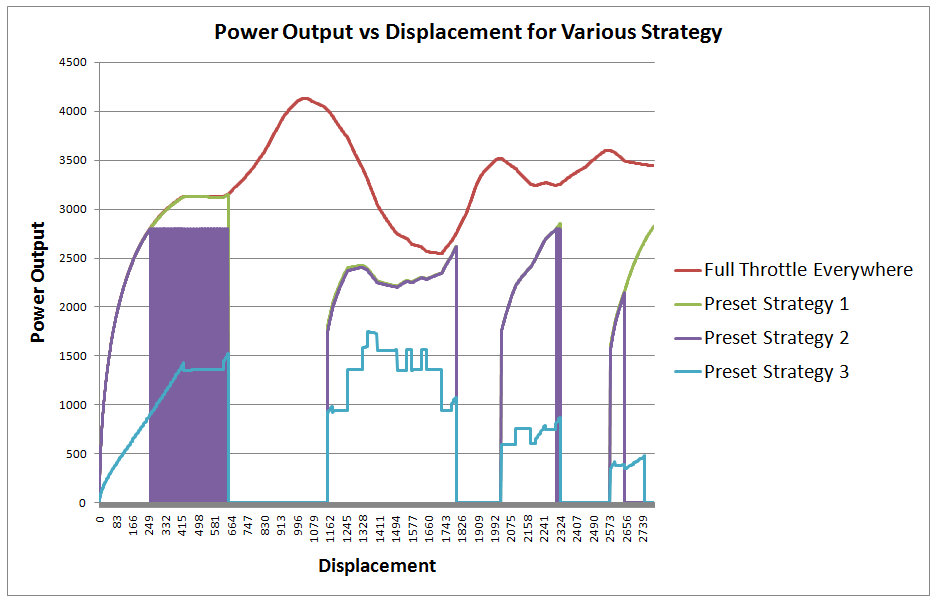
\includegraphics[width=4in]{images/power3.png}
	\caption{Graph of power output versus displacement for various strategy}
	\label{im:powerDisp}
	\end{figure}
}

\frame {
	\frametitle{Comparison Between Strategies}
	\begin{figure}[htb]
	\centering
	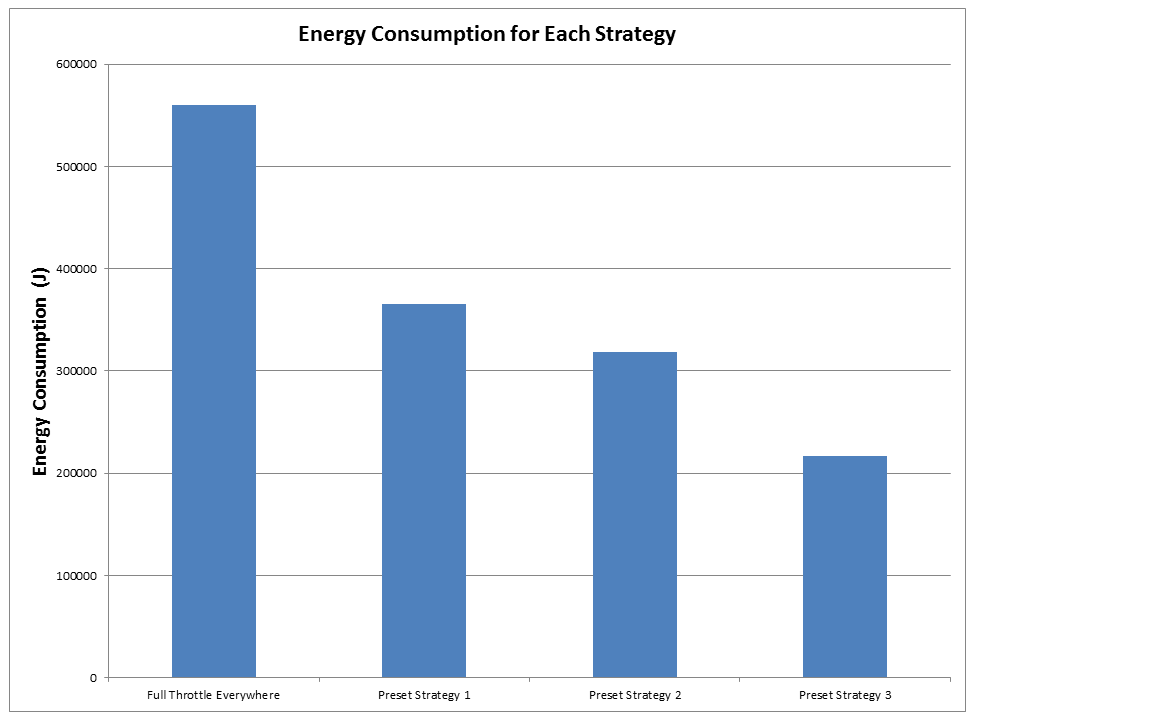
\includegraphics[width=4in]{images/energy.png}
	\caption{Graph of energy consumption for each strategy}
	\label{im:energyHist}
	\end{figure}
}

\frame {
	\frametitle{Comparison Between Strategies}
	\begin{figure}[htb]
	\centering
	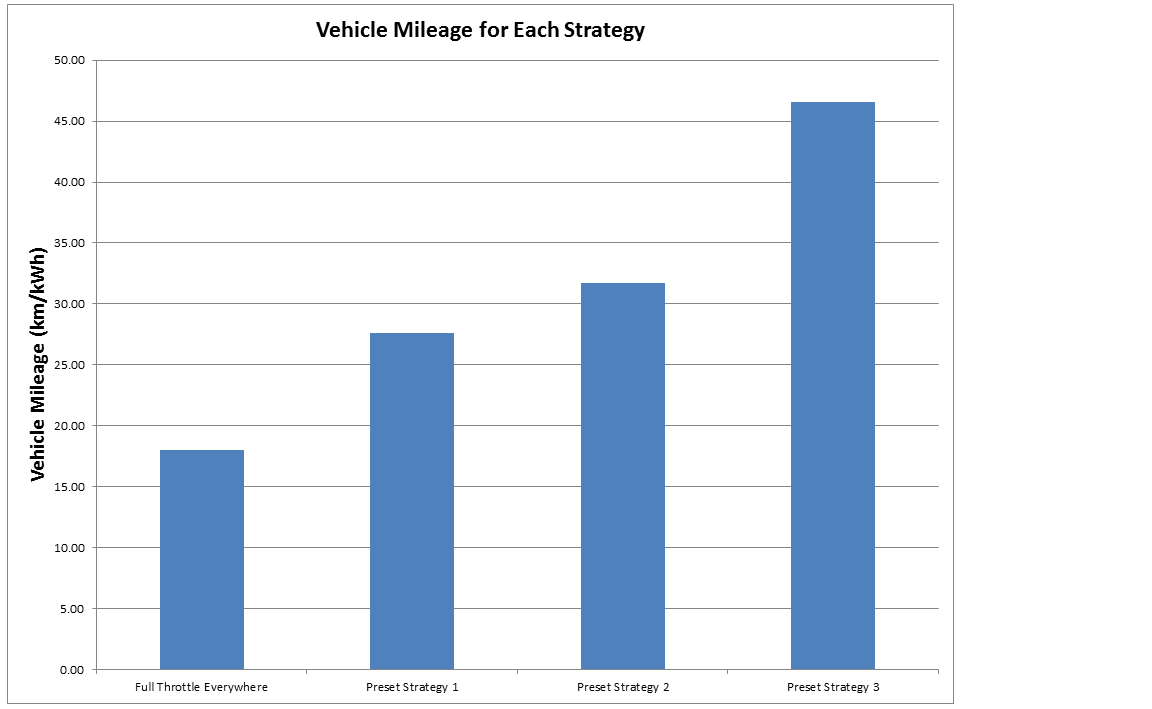
\includegraphics[width=4in]{images/mileage.png}
	\caption{Graph of vehicle mileage for each strategy}
	\label{im:mileageHist}
	\end{figure}
}

\frame {
	\frametitle{Comparison Between Strategies}
	\begin{figure}[htb]
	\centering
	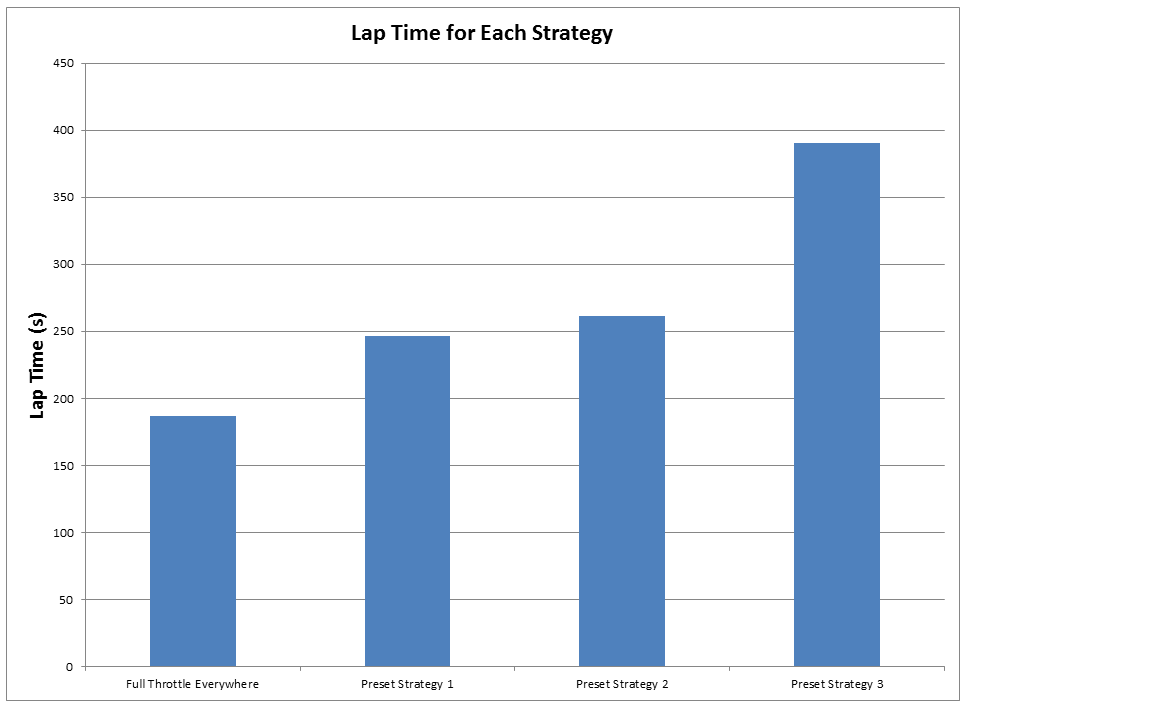
\includegraphics[width=4in]{images/laptime.png}
	\caption{Graph of lap time for each strategy}
	\label{im:laptimeHist}
	\end{figure}
}

\section{Conclusion}

\subsection{Conclusion}
\frame {
	\frametitle{Conclusion}
	\begin{enumerate}
		\item To identify the output signal of the controller circuit and the hall effect sensor of the PMBLDC and develop a set of instrument for measuring the mileage of the electric vehicle.  \textbf{(Achieved)}
		\item To study the track profile of Sepang North Track and create a simulation program for simulating the vehicle dynamics at the Sepang North Track. \textbf{(Achieved)}
		\item To compose a set of strategy to increase the mileage of the electric vehicle running on the Sepang North Track using the simulation program. \textbf{(Achieved)}
	\end{enumerate}
}

\subsection{Future Work}
\frame {
	\frametitle{Future Work}
	\begin{enumerate}
		\item hall effect sensor signal - controller phase current
		\item improve Coefficient of Drag
		\item improve vehicle simulation software
	\end{enumerate}
}

\frame {
	\Huge
	\centerline{Q\&A}
}

\frame {
	\Huge
	\centerline{Thank you}
}

\end{document}
